% !TeX program = lualatex
% PREVIEW BUILD: Introduction -> Institutional background -> Data only.
% The full paper is main.tex; this file is a partial preview and is not the submission.
%----------------------------------------------------
\documentclass[12pt,letterpaper]{article}
\usepackage{YGTemplate}

% Title
%----------------------------------------------------
\title{A Firm-Level Microsimulation for VAT Policy Analysis\thanks{\textbf{Acknowledgements:} I thank Max Ghenis and Seyed Mahdi Hosseini for their great suggestions and helpful discussions.}}
\author{Vahid Ahmadi\thanks{Research Associate at PolicyEngine. Email: \href{mailto:vahid@policyengine.org}{vahid@policyengine.org}} \\[0.4cm] \normalsize PolicyEngine}
\date{{\footnotesize\textcolor{red}{Preliminary and Incomplete. Comments are welcome.}} \\ \vspace{0.3cm} \small \ifcase\month\or January\or February\or March\or April\or May\or June\or July\or August\or September\or October\or November\or December\fi\ \the\year}

% Main document
%------------------------------------------------------
\begin{document}
\maketitle

\begin{abstract}
I present an open, reproducible firm-level microsimulation for pricing reforms to the UK VAT registration threshold, released in full---including its synthetic data generator---as open-source code. The threshold is a \emph{notch}: once turnover crosses \pounds85{,}000, 20\% VAT falls due on a firm's entire turnover rather than only the excess, creating an incentive to bunch below. I build synthetic firm-level records from ONS business-structure counts (sector $\times$ turnover band $\times$ employment), calibrate them to HMRC VAT statistics for 2023--24, and apply three tools: a static costing of threshold-location reforms, a reduced-form bunching estimator, and a calibrated Kleven--Waseem notch model for schedule-shape reforms the reduced form cannot price. I treat the model as a turnover-tax-notch approximation for consumer-facing, limited-reclaim firms, abstracting from input reclaim and voluntary registration. Static costing reproduces HMRC's published figure for the \pounds85{,}000 to \pounds90{,}000 reform ($-$\pounds175m versus $-$\pounds185m in 2025--26). Behavioural responses are small: bunching ratio $b\approx0.061$; median local turnover elasticity $\approx0.17$. I report each reform's static cost and how much of the \pounds21{,}250 dominated region it removes: raising the threshold to \pounds100k ($-$\pounds374m) leaves the \pounds21{,}250 zone, relocated; a banded 10\% reduced rate ($-$\pounds357m) reduces it to \pounds9{,}444; a 15\% reduced rate ($-$\pounds178m) reduces it to \pounds15{,}000; and a graduated taper over $[\pounds85\text{k},\pounds105\text{k}]$ ($-$\pounds335m) removes it.
\end{abstract}

\vspace{0.3cm}
\noindent\textbf{Keywords:} value-added tax, microsimulation, tax notch, policy

\newpage
\section{Introduction}\label{sec:intro}

The United Kingdom's Value Added Tax (VAT) applies above a registration threshold that is the highest in the OECD alongside Switzerland \citep{hoc_vat,hmrc_threshold}. The threshold is a \emph{notch} rather than a kink: once a firm's annual taxable turnover crosses it, VAT falls due on the firm's whole base, not only on the part above the threshold, so registration produces a discrete jump in liability rather than a marginal one. The threshold falls in a dense part of the firm distribution. Figure~\ref{fig:dist}(a) shows that VAT- and PAYE-registered UK businesses are concentrated at the lower end of the turnover distribution, and Figure~\ref{fig:dist}(b) shows that the VAT-registered population per \pounds1{,}000 of turnover is densest at and below the threshold, so the notch applies to a large number of firms.

\begin{figure}[htbp]
\centering
\subfigure[VAT- and/or PAYE-registered businesses (ONS, 2023--24)]{
    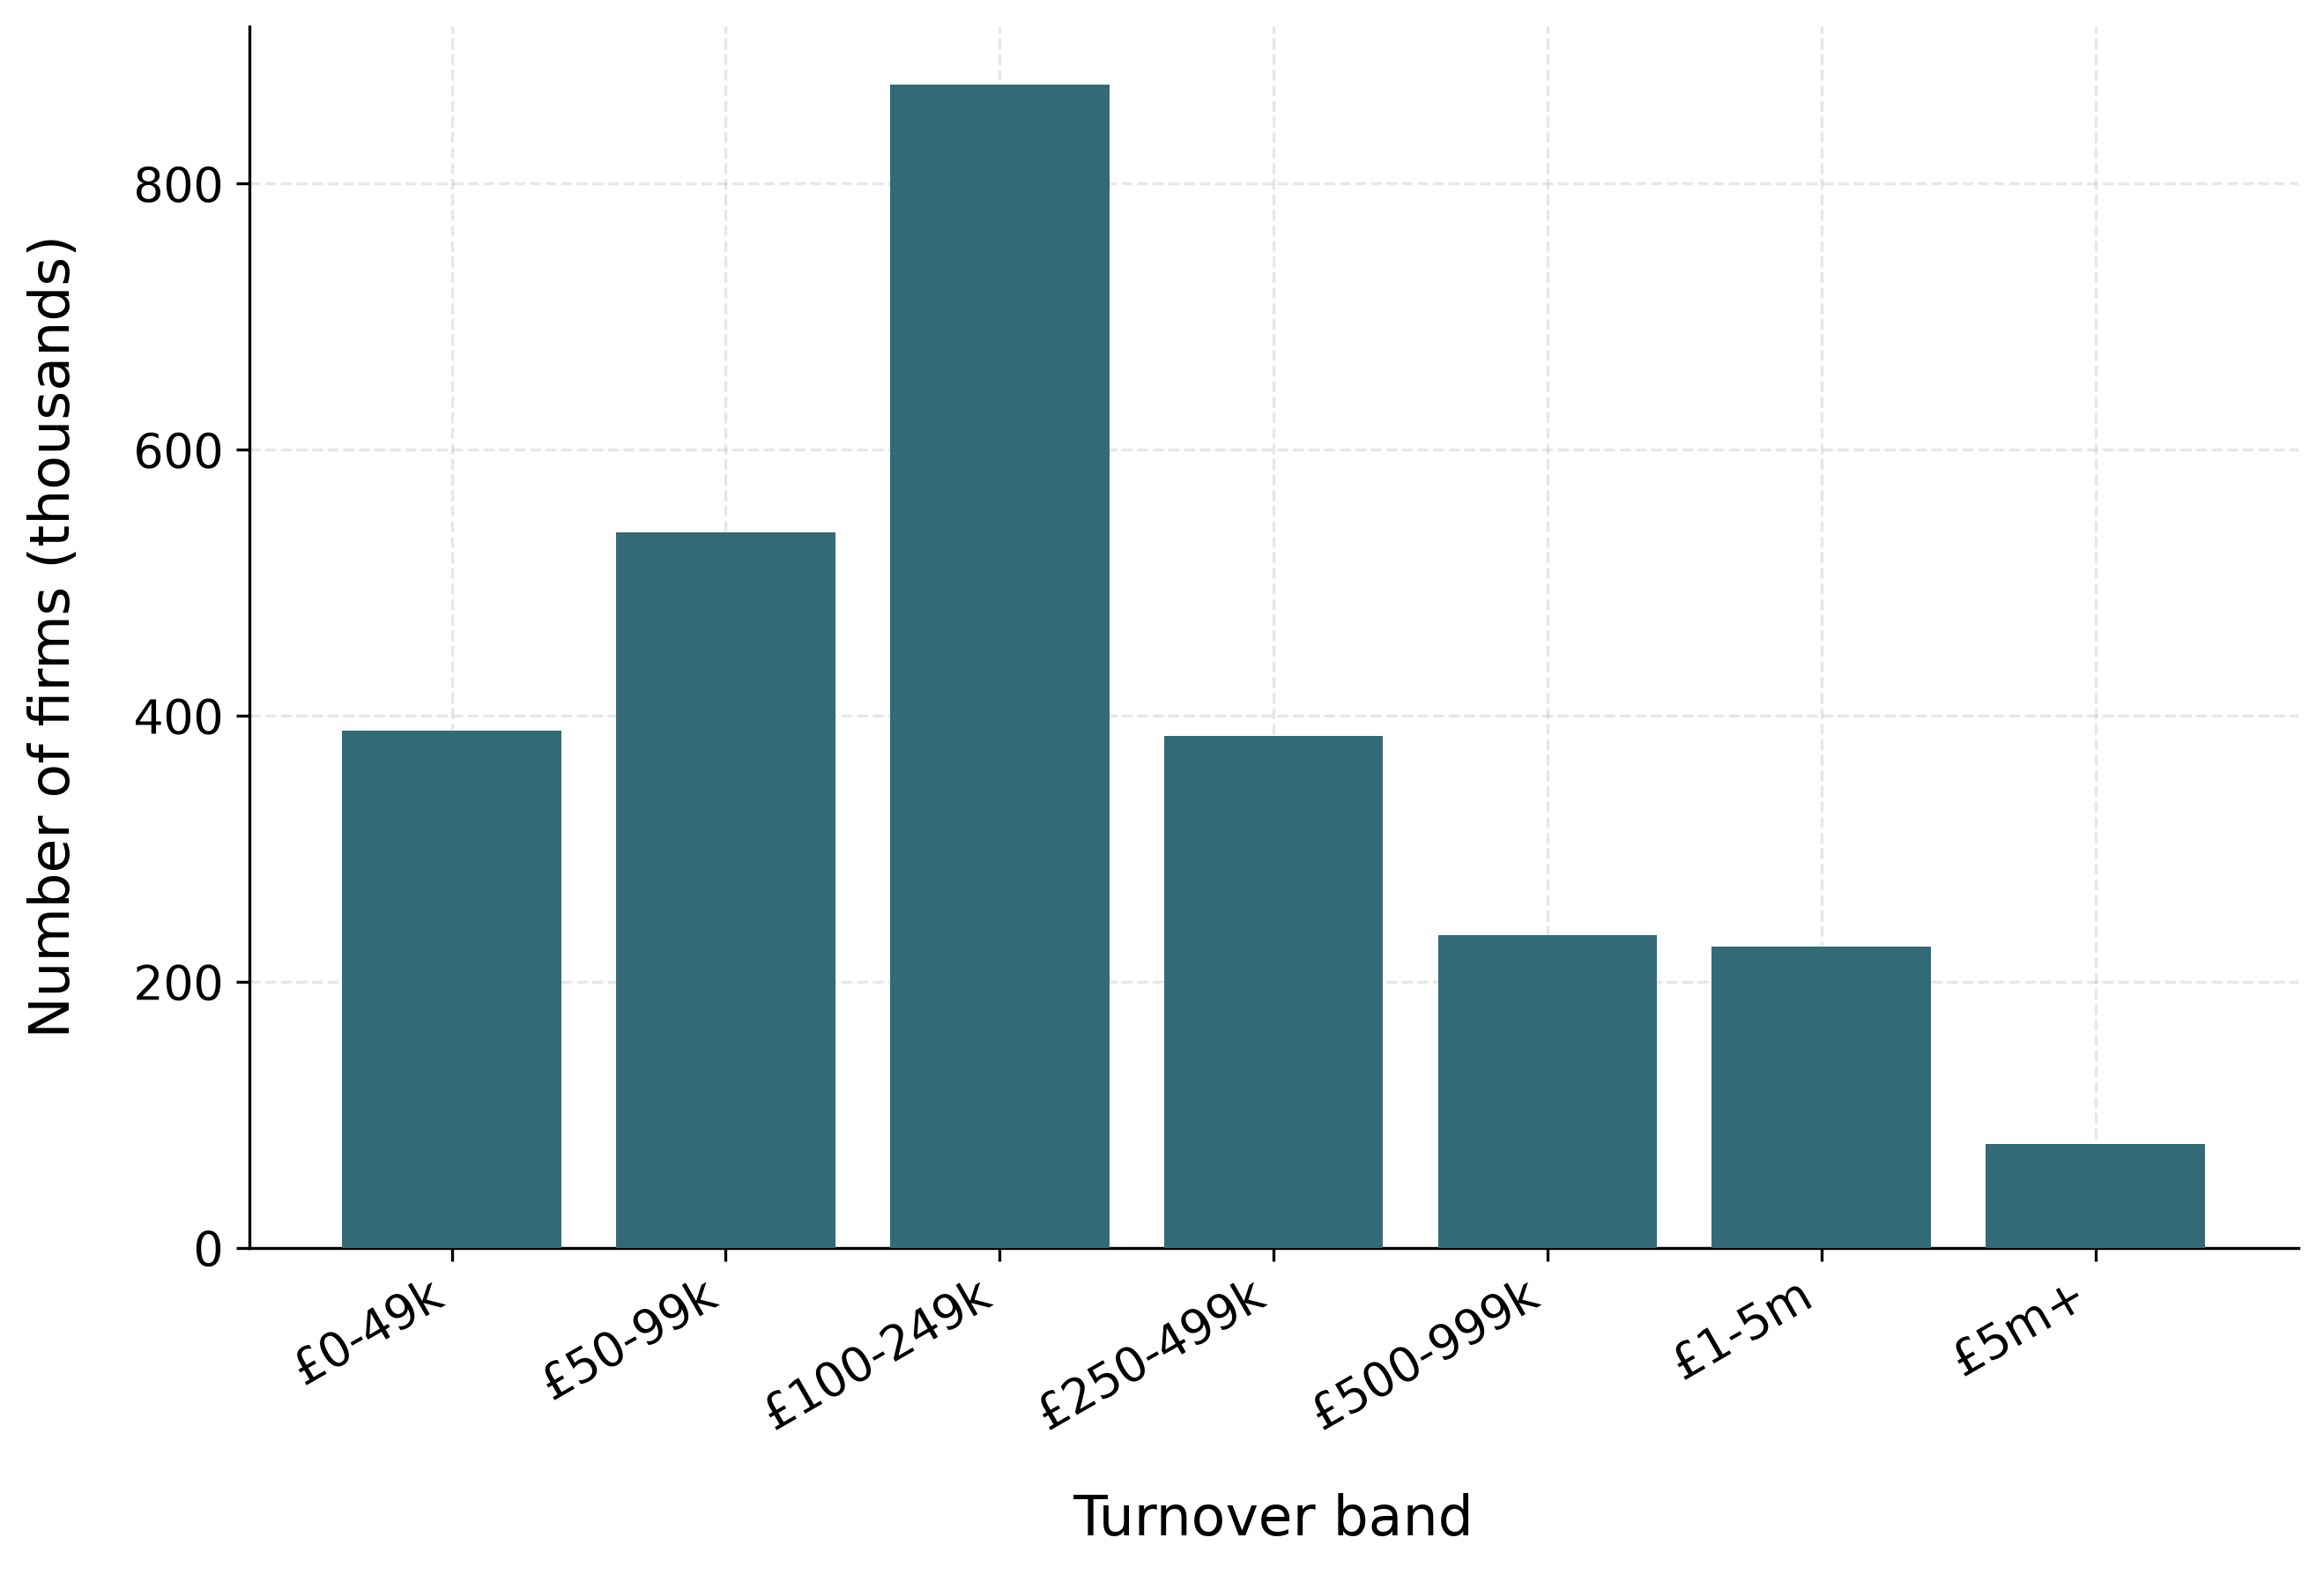
\includegraphics[width=0.48\textwidth]{figures/firms_by_turnover_band_85k.png}
}
\hfill
\subfigure[VAT-registered firms (HMRC, 2023--24)]{
    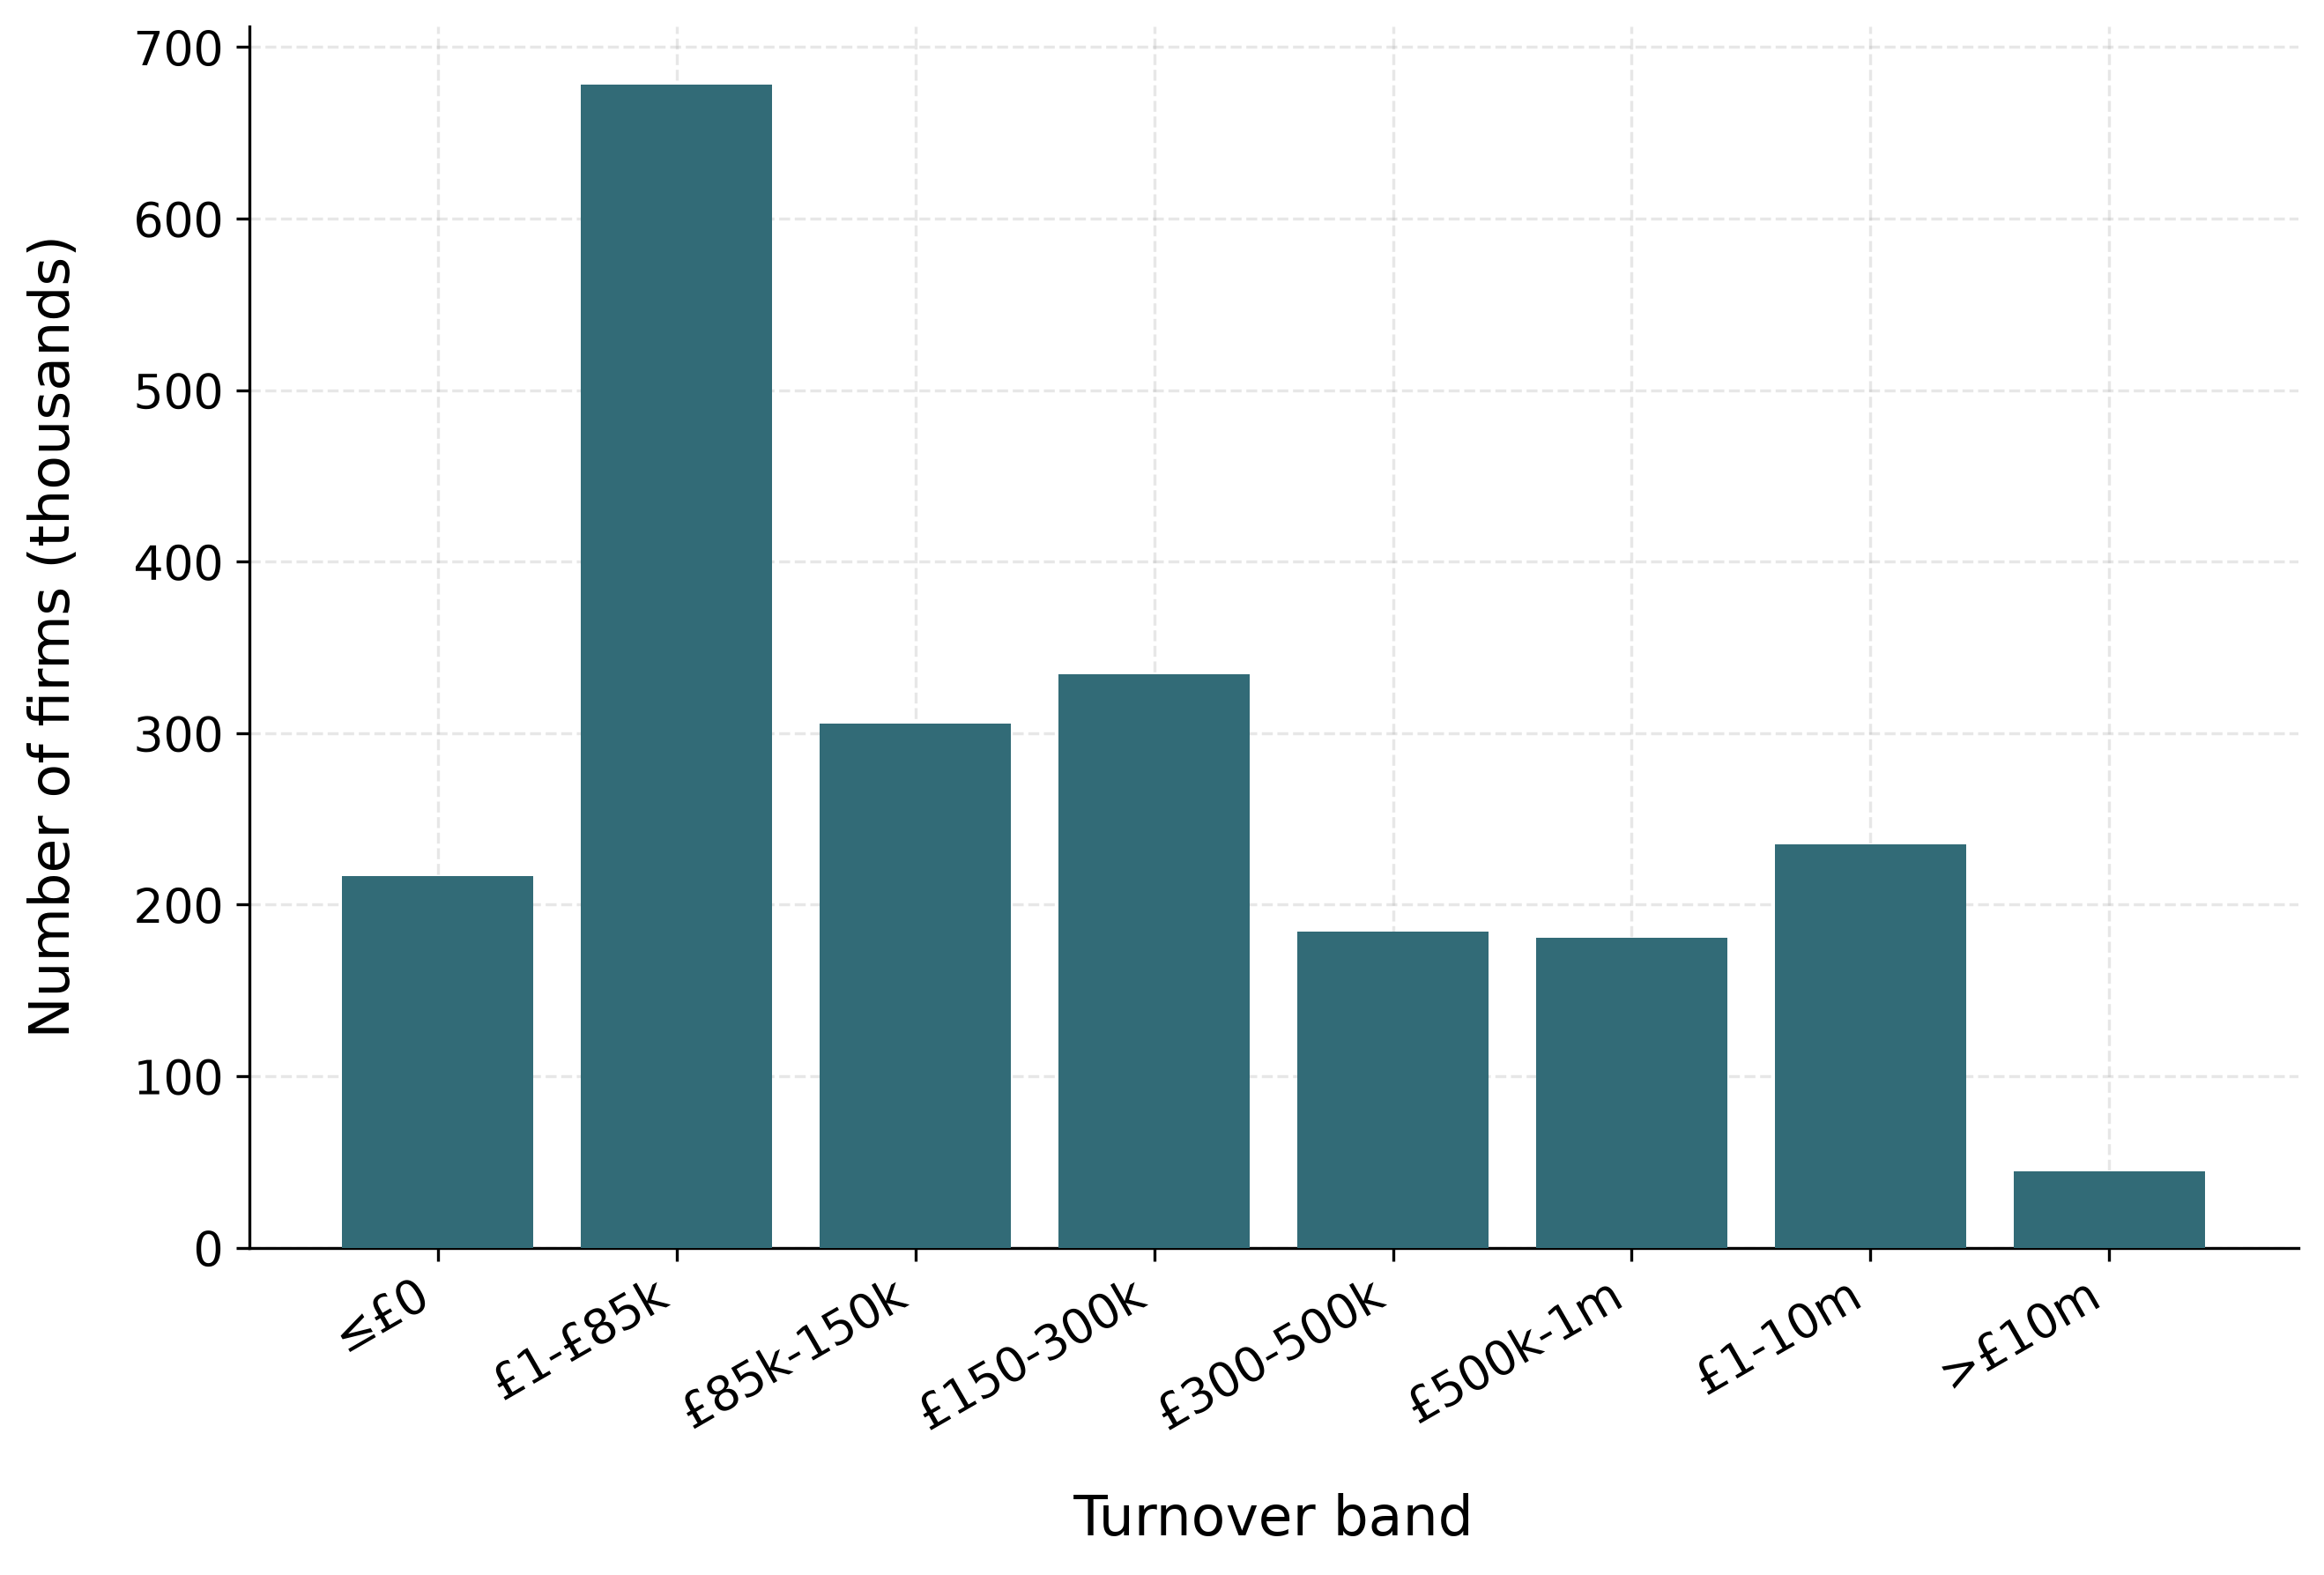
\includegraphics[width=0.48\textwidth]{figures/vat_firms_by_turnover_band_85k.png}
}
\caption{The UK firm-size distribution and VAT registration, 2023--24 (threshold
\pounds 85{,}000). Panel (a): number of businesses by turnover band in the ONS
business register, which covers businesses registered for VAT and/or PAYE
(about 2.7 million); the full business population including unregistered
businesses is roughly twice as large (DBT business population estimates).
Panel (b): number of VAT-registered firms by turnover band. Band widths are
unequal, so cross-band count comparisons should be read per \pounds1{,}000 of
turnover. Source: panel (a), ONS,
\href{https://www.ons.gov.uk/businessindustryandtrade/business/activitysizeandlocation/bulletins/ukbusinessactivitysizeandlocation/2023}{\emph{UK Business: Activity, Size and Location}}
(business counts by turnover band); panel (b), HMRC,
\href{https://www.gov.uk/government/statistics/value-added-tax-vat-annual-statistics}{\emph{Value Added Tax (VAT) Annual Statistics}}
(VAT-registered population by turnover band).}
\label{fig:dist}
\end{figure}

Firms respond to the notch by locating below the threshold. Tabulations of HMRC turnover
data show the number of firms rising towards \pounds 84{,}000 and then dropping sharply at
the \pounds 85{,}000 threshold, leaving excess mass just below it \citep{obr2023vat}.
\citet{liuetal2021} document this bunching in UK administrative firm data over
2004--05 to 2014--15, when the threshold rose from \pounds58{,}000 to
\pounds81{,}000, and \citet{liulockwoodtam2024}
find that firms slow their turnover growth as they approach the threshold. The notch
therefore distorts the size distribution and the growth decisions of firms near the margin,
which places the threshold under recurrent pressure for reform.

Reform proposals change the threshold in one of three ways: its \emph{level} (raising or lowering it), its \emph{shape} (replacing the notch with a schedule that phases the rate in over a band), or its \emph{rate} (a reduced rate for firms in a band above the threshold). The three are not equivalent. Changing the level moves the notch along the turnover axis; changing the shape or the rate alters the size of the discrete jump itself. Costing the three on a common basis is the practical difficulty this paper addresses. A change in the level can be costed by mechanical accounting, but a change in the shape of the schedule cannot be evaluated with the reduced-form bunching methods used to study the threshold, because a continuous schedule leaves no single point of excess mass to exploit. The firm-level data needed to study turnover near the threshold is, in addition, not available in open form.

In this paper I build an open, reproducible firm-level microsimulation for costing UK VAT threshold reforms on a common static basis. I construct synthetic firm microdata calibrated to published official aggregates---HMRC registered-firm counts by turnover band and by sector, net VAT liability by turnover band, and ONS business counts and employment bands---for the 2023--24 tax year, when the threshold was \pounds 85{,}000, and separately for 2024--25, when it rose to \pounds 90{,}000. Each firm's net VAT liability is the standard rate applied to its value added. The synthetic data can be released openly and regenerated under any counterfactual schedule.

On these data I do four things. First, I cost level reforms and schedule reforms---a graduated taper and a reduced-rate band---statically, by applying each counterfactual schedule mechanically to the firm distribution. Second, I characterise the notch's distortion through its \emph{dominated region}---the exact, elasticity-free range of turnover above the threshold in which no firm profits from locating---and how each reform changes it. Third, I price the level and rate reforms behaviourally: each firm re-optimises its turnover within its schedule region, conditional on an assumed turnover elasticity $e$ that the data do not identify, reported as an $e$-sensitivity range that nests the static costing exactly in its $e\to0$ limit. Fourth, I show that the synthetic data's near-threshold structure is target-inherited and cannot support bunching inference: the \pounds85{,}000 profile is calibrated to the OBR's published \pounds1{,}000-band data and the estimator reads exactly that back, a placebo without the fine targets returns zero, and the uncalibrated \pounds90{,}000 vintage shows a spurious band-edge signal.

Four findings follow. First, the static pipeline prices all the reforms on a common basis, and its anchor costing tracks the Government's published number once the deregistration convention is stated. My static costing of the April 2024 increase from \pounds 85{,}000 to \pounds 90{,}000 depends on what released firms are assumed to do: if every firm in the band deregisters, the 2025--26 cost is \pounds 323m, overshooting HMRC's published \pounds 185m \citep{hmt_spring_budget_2024} in line with the official costing's phased registration response; if the roughly 43\% voluntary-registration share that \citet{liuetal2021} document is retained, it is \pounds 184m---matching the published figure to \pounds 1m. Both conventions reproduce the official profile's narrowing and its 2028--29 sign change. Forward moves from the \pounds 90{,}000 base range from a gain of about \pounds 1{,}040m at \pounds 70{,}000 to a cost of about \pounds 1{,}450m at \pounds 120{,}000, against a base of about \pounds 200.9bn in 2025--26.

Second, the shape and rate reforms act on the notch's distortion in a way that a change in level does not. The notch creates a \emph{dominated region} of width $a = T^{*}\tau/(1-\tau) = \pounds 21{,}250$ above the threshold (\pounds 85{,}000--\pounds 106{,}250), a range of turnover in which no firm can locate without being strictly worse off than at the threshold. This region is an exact property of the schedule: under the value-added formulation of Section~\ref{sec:behavioural} its width is the same for every firm with positive value added, whatever its input share, and it requires no behavioural calibration. It also spans a populous part of the firm distribution---about 156{,}000 weighted firms in the calibrated data---so its width is an economically meaningful distortion index. Raising the threshold relocates this region without removing it. A reduced rate does \emph{not} remove it: the jump at the threshold falls (from \pounds 17{,}000 to \pounds 12{,}750 at a 15\% band), but the band reverts to the standard rate at its \pounds 105{,}000 top, introducing a second notch and a second dominated region, so the total dominated width is essentially unchanged---\pounds 21{,}562 at 15\% and \pounds 22{,}569 at 10\%, both marginally above the \pounds 21{,}250 baseline. Only the graduated taper, being continuous, removes the dominated region. On the common \pounds 85{,}000 data-year base, raising the threshold to \pounds 100{,}000 costs \pounds 753m and removes none of the dominated region; the taper removes all of it for \pounds 520m; and the 10\% and 15\% reduced rates cost \pounds 484m and \pounds 242m while splitting the dominated band in two. On the dominated-region metric the level move is the most expensive option per unit of distortion removed---a comparison that indexes the misallocation distortion only and omits the compliance-cost saving a higher threshold delivers (Section~\ref{sec:conclusion}).

Third, conditional on the assumed elasticity, intensive-margin responses barely move these costings. A pure level rise has \emph{exactly} zero intensive-margin revenue offset at every $e$: released firms leave the VAT base, so their expansion is untaxed, and no other firm's effective rate changes---a result the simulator verifies to \pounds0.1m. For the reduced-rate bands the offset is second order: at $e=0.17$ the 10\% band's cost falls from \pounds 484m to \pounds 475m and the 15\% band's from \pounds 242m to \pounds 235m, under 6\% even at $e=0.32$. I do not report a behavioural cost for the graduated taper: its rate varies continuously with turnover, so its marginal-rate channel is outside the flat-rate machinery, and only its static cost and dominated-region removal are reported. The sweep values $e \in \{0.05, 0.17, 0.32\}$ are assumptions: the lower end has an external anchor \citep{klevenwaseem2013}, and the published UK VAT-base estimates of \citet{liuetal2021} fall between it and the midpoint. The consequence of these results runs opposite to the usual worry: the static costings are robust to the intensive margin, and the behavioural uncertainty that matters---registration and location choice at the notch---is exactly the margin the synthetic data cannot identify.

Fourth, the open data carry a transparency lesson about bunching: every sub-band feature of band-calibrated synthetic data is exactly what its targets put there, and this paper demonstrates the point in three directions. The 2023--24 population's near-threshold density is calibrated to the OBR's published \pounds1{,}000-band profile \citep{obr2023vat}, so it reproduces the administratively observed bunching shape---and the estimator reads that shape back as excess mass ($E=7{,}933$), which is target inheritance, not behaviour. A placebo that regenerates the population \emph{without} the fine targets returns $E=0$: remove the targets and the ``bunching'' vanishes. And the 2024--25 vintage, for which no fine bands are published, shows what the trap looks like from the other side: the coarse \pounds90{,}000 band edge alone produces an excess-bunching statistic within 10\% of the administrative estimate of \citet{liuetal2021}---a coincidence of band geometry, four-fold unstable across estimator specifications, with no behaviour behind it. An earlier draft of this paper reported ``reproducing'' the administrative step when a liability mis-scaling in the generator manufactured it; the correction removed it, and the OBR targets now supply the shape from published data instead. The lesson is symmetric and general: synthetic bunching is not evidence of behaviour, its absence is not evidence of no behaviour, and any sub-band feature of calibrated data should be traced to its targets before it is read as economics. The behavioural evidence on UK VAT bunching remains \citeauthor{liuetal2021}'s administrative estimate.

\subsection*{Related literature}

The paper draws on four strands of work. The first is the methodology of bunching and notches \citep{chettyetal2011,saez2010,klevenwaseem2013,kleven2016,best2015}, which provides the analytic notion of a dominated region; I use the dominated region to characterise a distortion that leaves no single point of excess mass to exploit.

The second is the empirical literature on VAT registration thresholds \citep{liuetal2021,liulockwoodtam2024,onji2009,harju2019,asatryanpeichl2017,nandiwarwick2020,waseem2024}. \citet{liuetal2021} is closest: it estimates bunching at the UK notch on administrative data over 2004--2014 and documents voluntary registration; I take its estimates as the established behavioural facts and cost shape and rate reforms statically on a common basis, which that literature does not do. The international evidence \citep{harju2019,onji2009,asatryanpeichl2017,nandiwarwick2020} notes that bunching at a VAT threshold can reflect compliance costs, firm-splitting, or reporting rather than real turnover responses.

The third strand questions whether bunching identifies a structural elasticity at all: \citet{blomquistetal2021} show that the elasticity is not non-parametrically identified from bunching at a kink or a notch without strong functional-form assumptions, and \citet{bertanhaetal2023} develop the notch case. This literature motivates my refusal to read an elasticity off the synthetic data: even setting aside the placebo evidence that any synthetic step is mechanical, the mapping from excess mass to an elasticity requires assumptions I am unwilling to impose. The fourth strand is the structural literature on size-based thresholds \citep{garicano2016,gourioroys2014}, which identifies policy-invariant primitives at the French 50-employee threshold and computes welfare from them; the present paper makes no such structural claim.

This paper makes three contributions. First, it provides an open, reproducible firm-level microsimulation for costing UK VAT threshold reforms, where the existing firm-level evidence rests on restricted administrative data; the released pipeline regenerates every number in the paper from public inputs. Second, it characterises the notch's distortion through its exact dominated region and costs two schedule reforms---a graduated taper and a reduced-rate band---on the same static basis as level reforms. Third, it demonstrates, by construction and by correction, that band-calibrated synthetic data carry no sub-band behavioural information beyond their targets: the paper documents how its own earlier build manufactured a plausible-looking density step, how the correction removed it, how calibrating to the OBR's published fine bands restores the administrative shape as an explicit target, and how the same band-edge mechanism manufactures a spurious signal where no fine targets exist. Identifying the turnover elasticity from administrative micro-data, a welfare accounting, revenue-neutral designs, and an explicit model of voluntary registration are left for future work.

The remainder of the paper proceeds as follows. Section~\ref{sec:background} describes the institutional background of the UK VAT threshold. Section~\ref{sec:data} sets out the synthetic firm microdata and its calibration to official aggregates. Section~\ref{sec:static} sets out the static costing of threshold changes and the schedule reforms. Section~\ref{sec:bunching} shows that the synthetic data contain no usable bunching signal and validates the estimator's power on injected signals. Section~\ref{sec:model} develops the notch and its exact dominated region, and shows how each reform changes it. Section~\ref{sec:behavioural} prices the reforms behaviourally, conditional on an assumed elasticity, and derives the level-rise invariance. Section~\ref{sec:conclusion} concludes.

\section{Institutional background}
\label{sec:background}

\paragraph{Registration and the notch.} The United Kingdom levies a value-added
tax at a standard rate of 20\% on most goods and services. A business must
register once its taxable turnover over any rolling twelve-month period exceeds
the registration threshold, after which it charges VAT on its taxable sales and
reclaims VAT paid on inputs. Because registration makes VAT due on the firm's
\emph{entire} taxable turnover rather than only the amount above the cutoff, the
threshold is a \emph{notch}---a discrete jump in liability---and not a kink. The
cost of crossing is largest for consumer-facing firms with limited pass-through
and small reclaimable input shares, for whom the incentive is to restrain
turnover and locate just below the threshold \citep{liuetal2021,klevenwaseem2013}.

\paragraph{Value added, input reclaim, and voluntary registration.} Real VAT is a
tax on \emph{value added}, not on turnover: a registered firm charges output VAT
on its sales but reclaims input VAT on its purchases. The model reflects this:
each synthetic firm's net liability is the standard rate applied to its value
added (Section~\ref{sec:data}), and under the value-added formulation the
notch's dominated region is invariant to the firm's input share
(Section~\ref{sec:model}). Two features of the real system remain outside the
model's scope. A large share of below-threshold firms register
\emph{voluntarily}---roughly $43\%$ of eligible below-threshold firms
\citep{liuetal2021}, driven by input-VAT reclaim and business-to-business
sales---and for them the threshold carries no bunching incentive; voluntary
registration enters the model only as a registration-rate parameter and a
retention sensitivity, not as a choice. And net-repayment traders (zero-rated
exporters and similar, HMRC's negative-liability column) are not represented,
because the public aggregates do not resolve rated structure by turnover band.

\paragraph{Threshold history.} The registration threshold was held at
\pounds85{,}000 from 1~April 2017 to 31~March 2024---a seven-year nominal freeze,
the longest in the history of the tax---before being raised to \pounds90{,}000 on
1~April 2024, with the deregistration threshold rising from \pounds83{,}000 to
\pounds88{,}000 \citep{hmrc_threshold,hoc_vat}. Because nominal turnover grows
with inflation and real activity, freezing the threshold lowers it in real terms
and draws an increasing number of firms towards the registration margin; this
fiscal-drag mechanism was a central motivation for the April~2024 increase. My
data year is 2023--24, so the prevailing statutory threshold throughout my
analysis is \pounds85{,}000. Figure~\ref{fig:obr_bunching} shows the pattern in
the turnover distribution: the number of firms rises towards \pounds84{,}000 and
falls sharply above \pounds85{,}000, and the projected 2025--26 distribution is
more sharply bunched than the 2019--20 outturn as fiscal drag draws more firms
towards the frozen threshold.

\begin{figure}[htbp]
\centering
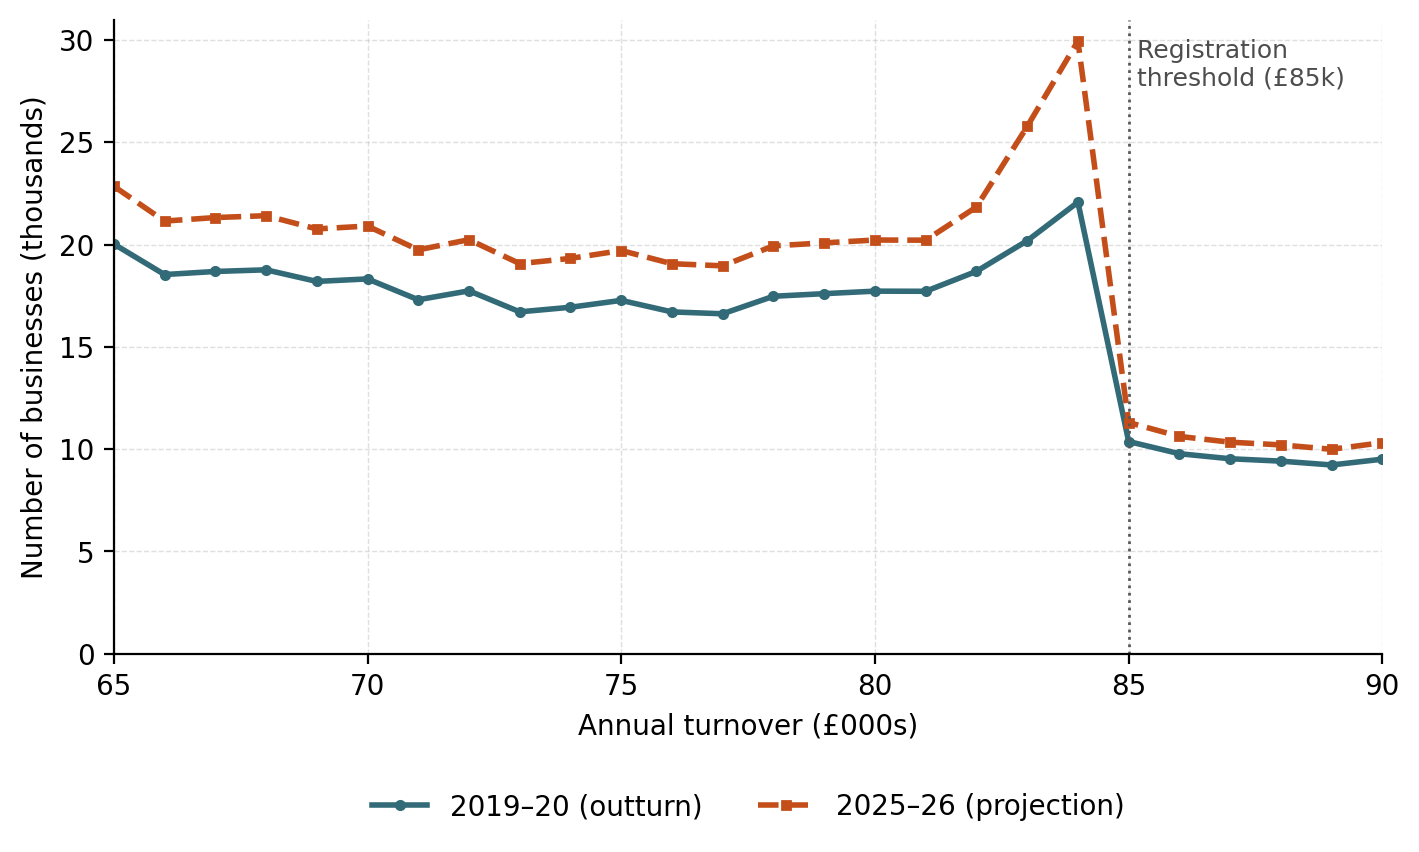
\includegraphics[width=0.74\textwidth]{figures/obr_vat_bunching_85k.png}
\caption{Bunching below the \pounds85{,}000 VAT registration threshold: number of
businesses by \pounds1{,}000 turnover band. Source:
\href{https://obr.uk/box/the-impact-of-the-frozen-vat-registration-threshold/}{OBR,
\emph{Economic and Fiscal Outlook} March 2023}, Chart C (Open Government Licence).}
\label{fig:obr_bunching}
\end{figure}

\paragraph{The reform debate.} The UK threshold is the highest in the OECD
alongside Switzerland \citep{hmrc_threshold},
and there is debate over whether to raise it---to reduce the compliance burden on
small firms---or lower it, to broaden the base and reduce the growth distortion at
the margin. Three families of reform feature, and I evaluate all three: a change in
the threshold's \emph{level} (the \pounds85{,}000 to \pounds90{,}000 increase
of April~2024 and further moves around it); a change in its \emph{shape} (a
\emph{graduated taper} that phases the effective rate in over a band, replacing the
notch with a continuous profile); and a change in its \emph{rate} (a \emph{reduced
rate} for small firms in a band above the threshold, with the standard 20\% rate
retained above). The taper and reduced-rate designs follow proposals in the UK
policy debate: \citet{ots2017vat} canvassed a financial incentive or reduced
effective rate to smooth the cliff-edge at the threshold, and HM Treasury's
call for evidence on the registration threshold examined smoothing mechanisms
in the same family \citep{hmt2018cfe}. The European Union ran a closely
related ``graduated relief'' scheme for small enterprises and abolished it
from January~2025 on complexity grounds, in favour of a simple exemption with
a transition tolerance \citep{eudirective2020285}---relevant precedent for the
administrability of taper-style designs. A banded reduced rate introduces a
smaller \emph{secondary} notch at the band top, which the continuous taper
avoids. I cost all three by the same machinery in Section~\ref{sec:static}.

\section{Data}
\label{sec:data}

Studying firm responses at the threshold needs firm-level turnover near the
cutoff, which the official statistics publish only in coarse turnover bands. I
therefore build a synthetic firm population calibrated to those aggregates: it
reproduces the official totals while resolving the individual firm that the
authorities do not release, opening the analysis to anyone. The same
calibrate-to-published-aggregates approach underlies open household-level
tax-benefit microsimulation \citep{policyengine}; here I apply it at the firm
level. The generator takes the registration threshold as a parameter and is
documented in Appendix~\ref{app:data}; I build one population for 2023--24
(threshold \pounds85{,}000), the paper's primary data year, and one for
2024--25 (threshold \pounds90{,}000), used for the forward sweep of
Section~\ref{sec:static}.

The archived CSV inputs in this repository remain the reproduction source for
the paper's reported numbers; a pinned migration snapshot also represents the
same numeric target surface through PolicyEngine Ledger and the
experimental Populace firm generator, and Appendix~\ref{app:data} reports the
parity check between that shared source-of-truth path and the paper inputs.

\paragraph{Construction.} Index firms by $i$. For each sector $s$ and ONS
turnover band $b=[\underline{b},\overline{b}]$, the \emph{UK Business: Activity,
Size and Location} table gives a business count $N_{s,b}$, and I draw $N_{s,b}$
firms with within-band turnover
\[
  y_i \;=\; \underline{b} + (\overline{b}-\underline{b})\,u_i + \varepsilon_i,
  \qquad u_i \sim \mathcal{U}(0,1), \;\; \varepsilon_i \sim \mathcal{N}(0,\sigma_b^2),
\]
truncated below at zero, where $\varepsilon_i$ smooths the within-band
distribution. The ONS register covers businesses registered for VAT and/or
PAYE---about 2.7 million---so the synthetic population represents that
registered-business frame, not the full business population of roughly
5.6 million in the DBT business population estimates; the difference is
concentrated below the threshold and matters for threshold \emph{cuts}, which I
flag where relevant. Each firm is given input expenditure $x_i = \rho_i\,y_i$,
with the input--output ratio $\rho_i$ drawn from a rescaled Beta distribution
with sector-specific shifts, clamped to $\rho_i \in [0.1, 0.95]$ (mean about
0.6, so value added averages about 40\% of turnover, in line with the UK
non-financial business economy). Its net VAT liability is the standard rate
applied to its value added,
\[
  v_i \;=\; \tau\,(y_i - x_i), \qquad \tau = 0.20,
\]
so every firm's net rate $v_i/y_i = \tau(1-\rho_i)$ lies in $[1\%, 18\%]$,
strictly positive and below the statutory cap of 20\%. The model therefore
abstracts from net-repayment traders (firms with zero-rated outputs whose input
reclaim exceeds output VAT---HMRC's negative-liability column); representing
them requires rated-structure detail (zero, reduced, and exempt output shares)
that the public aggregates do not resolve by band. Employment is assigned from
the ONS employment-band shares.\footnote{An earlier draft of this generator set
$v_i = y_i - x_i$ with $\rho_i \in [0.6, 1.5]$---omitting the factor $\tau$, so
per-firm liabilities were about five times too large and a large minority of
firms carried negative value added. The weight optimiser compensated on the
band totals, leaving aggregate calibration scores similar but distorting the
near-threshold density; Section~\ref{sec:bunching} documents the consequence
and the correction.}

The base population reproduces the ONS structure but not
the HMRC VAT-registered totals, so I re-weight it. Each firm receives a strictly
positive weight $w_i = e^{\theta_i}$, and for a vector of official targets
$T=(T_k)_{k=1}^{K}$ the weighted synthetic counterpart of target $k$ is
\[
  \widehat{T}_k(\theta) \;=\; \sum_i a_{ki}\, w_i ,
\]
where $a_{ki}$ is firm $i$'s contribution to target $k$: an indicator of band or
sector membership for a count target, and the firm's net liability $v_i$ for a
VAT-liability target. I choose $\theta$ to minimise a symmetric relative-error
loss with per-target importance weights $\lambda_k$,
\[
  L(\theta) \;=\; \frac{1}{K}\sum_{k} \lambda_k
    \min\!\Big\{ \big(\widehat{T}_k/T_k - 1\big)^2,\; \big(T_k/\widehat{T}_k - 1\big)^2 \Big\}
    \;+\; \frac{\alpha}{N}\sum_i \lvert \theta_i \rvert ,
\]
the final term a mean absolute penalty on the log-weights. The targets are the
HMRC VAT-registered counts by turnover band and by sector, the HMRC net VAT
liability by turnover band, the ONS employment-band totals, and---for the
2023--24 vintage---the OBR's published near-threshold profile: the March 2023
\emph{Economic and Fiscal Outlook} Chart~C data give HMRC counts of businesses
by \pounds1{,}000 turnover band over \pounds65{,}000--\pounds90{,}000
\citep{obr2023vat}, which I interpolate to the 2023--24 data year between the
2019--20 outturn and the OBR's 2025--26 frozen-threshold projection. The five
bins at or above the threshold enter as direct count targets (every
firm there is VAT-registered, the same universe as the coarse HMRC band they
refine); the twenty bins below the threshold enter as \emph{shape} targets,
normalised over the \pounds65{,}000--\pounds85{,}000 window and scaled to the
synthetic population's own mass there, because the chart counts a narrower
universe than the ONS business frame below the threshold. These fine targets
pin the near-threshold density to the administratively observed bunching
profile---the region that coarse bands alone leave to the weight optimiser
(Section~\ref{sec:bunching}). No fine bands are published for the
\pounds90{,}000 threshold era, so the 2024--25 vintage keeps coarse bands
only. Turnover-band and near-threshold targets carry the largest $\lambda_k$,
followed by VAT liability by band. VAT liability by sector is reported as an
informational diagnostic but excluded from the optimizer, because the
generator draws a common input-share distribution with sector shifts rather
than calibrating the input/output tax structure by sector. The problem is
solved by gradient descent, and the symmetric loss keeps targets of very
different magnitudes on a common scale.

A firm is registered with certainty when its data-year turnover exceeds the
threshold $T^{*}$. This is an approximation to the statutory test, which is a
rolling 12-month test on \emph{taxable} turnover with a roughly two-month
registration lag, a forward-looking 30-day test, and an exception for temporary
breaches (Section~\ref{sec:background}); the model also registers firms whose
turnover is largely exempt, whom the law would not require to register. For a
single-year cross-section calibrated to registered-population totals these
timing and composition wedges are second order for the aggregates, but they are
worth naming: the HMRC band tables classify traders by total declared outputs
(VAT-return Box 6), and the ONS turnover measure is likewise total turnover, so
the running variable throughout is total rather than taxable turnover. Below
the threshold a firm registers voluntarily with probability $r = M / n_{<}$,
where $M$ is the HMRC count of registered firms in the \pounds1--threshold band
and $n_{<}$ is the unweighted number of synthetic below-threshold firm rows.
This sets the expected row-level voluntary-registration rate; I do not treat
below-threshold voluntary registration as a separate weighted calibration
target. The resulting dataset comprises approximately $2.94$~million firm
records per vintage, weighted to represent roughly $2.5$~million registered
businesses. Checked against the official sources along every calibrated
dimension, both vintages attain an overall calibration accuracy of 89.4\%,
with dimension scores ranging from 77.9\% (2023--24 employment bands) and
79.0\% (2024--25 liability by band) to 94.4\%; Appendix~\ref{app:data} reports
the full table. The headline is the mean of five calibrated-dimension scores,
each clipped at zero as $\max\{0,1-\lvert \widehat{T}-T\rvert/\lvert T\rvert\}$;
it excludes the VAT-liability-by-sector diagnostic described above.

\paragraph{The registration threshold in the data.} My primary data year is
2023--24, when the statutory threshold was \pounds85{,}000. The HMRC band
targets step down across the threshold---678{,}350 firms in the
\pounds1--\pounds85{,}000 band against 305{,}320 in
\pounds85{,}000--\pounds150{,}000, or roughly $8{,}000$ against $4{,}700$ firms
per \pounds1{,}000 of band width---and the calibrated population necessarily
inherits that band-average step. The \emph{local} shape within a few thousand
pounds of the threshold is pinned by the OBR near-threshold targets described
above: the calibrated density rises into the threshold (about $13{,}800$ firms
per \pounds1{,}000 in the \pounds84{,}000--\pounds85{,}000 bin), steps down
across it (about $11{,}500$ just above), and declines through the band---the
administratively observed bunching profile \citep{obr2023vat,liuetal2021},
present in the file because it is targeted, not because any synthetic firm
chooses it. In an earlier build without these targets the local shape was an
unpinned optimiser equilibrium (and, under the pre-correction liability scale,
a spurious bunching look-alike); the central data caveat of the paper stands
in all three configurations: no sub-band feature of band-calibrated synthetic
data carries behavioural information beyond what its targets put there
(Section~\ref{sec:bunching} quantifies this with placebo and recovery tests).
Counterfactual policies---including the \pounds85{,}000 to \pounds90{,}000
reform and the forward threshold sweep of Section~\ref{sec:static}---are
evaluated on these firms by re-applying the registration rule to the microdata
for the static costings, holding the empirical turnover distribution fixed. A
behavioural layer that re-prices firms under counterfactual schedules,
conditional on an assumed turnover elasticity, is developed in
Section~\ref{sec:behavioural}.

\begin{figure}[htbp]
\centering
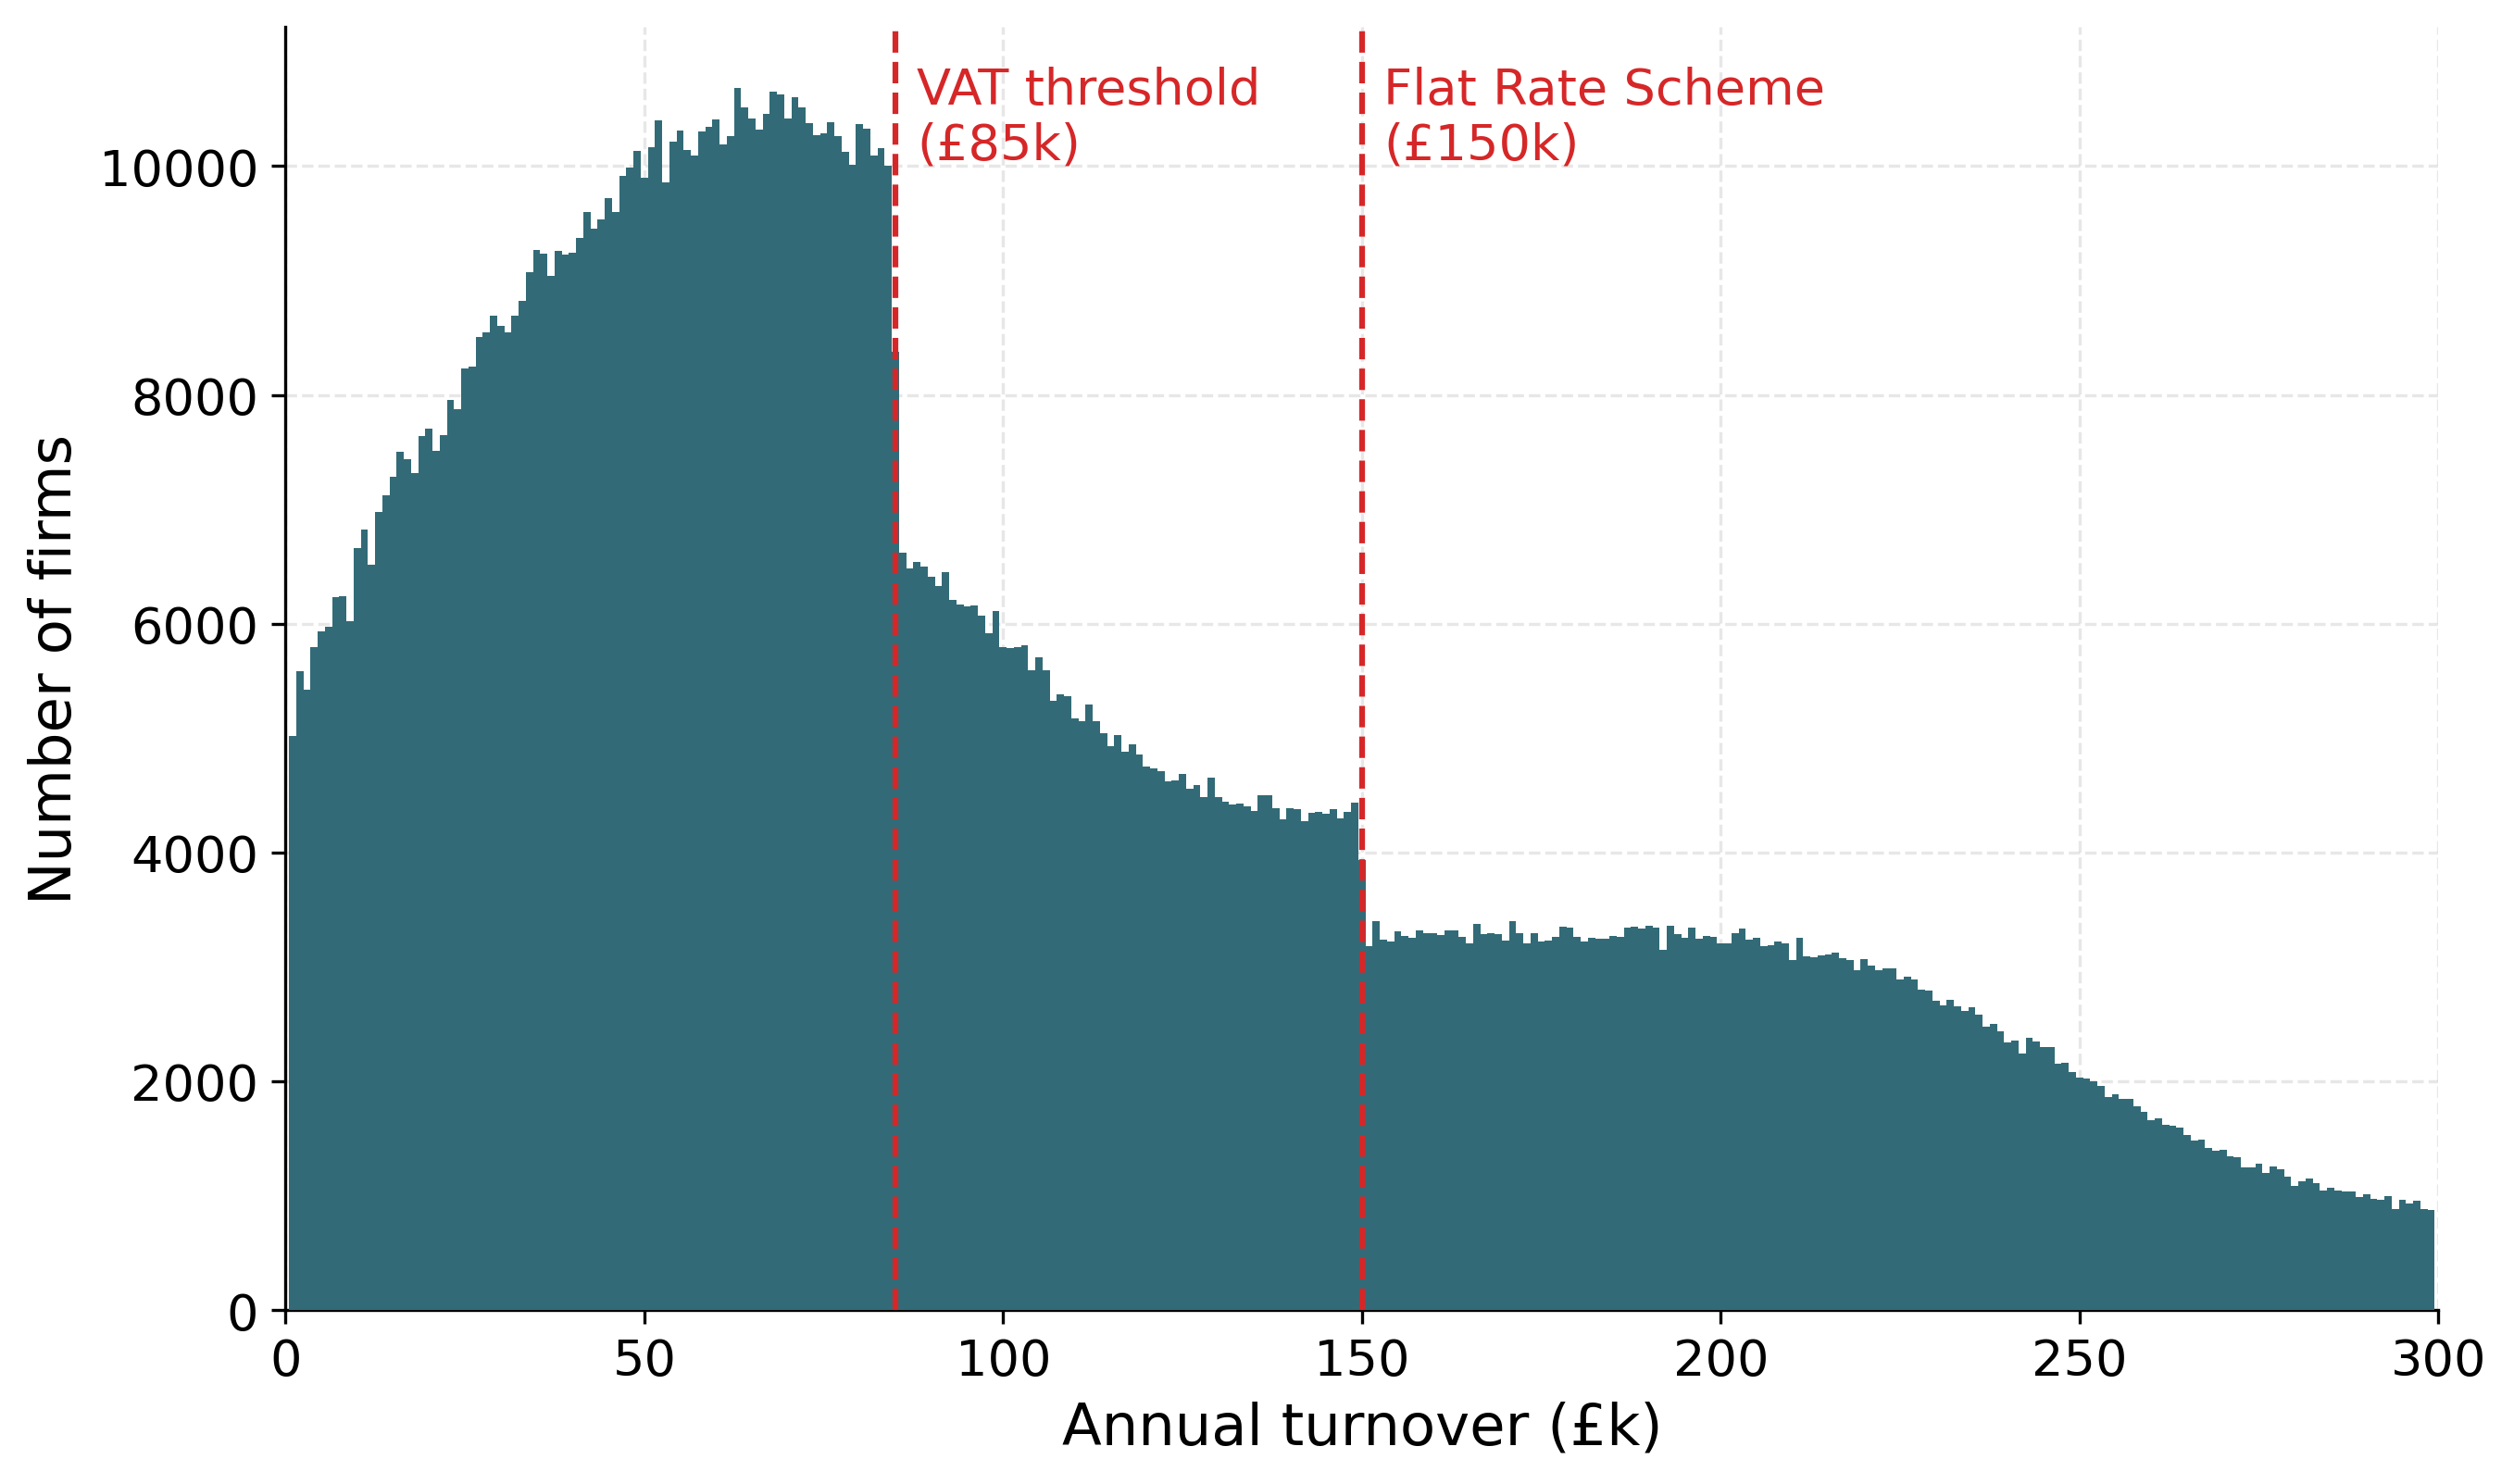
\includegraphics[width=0.74\textwidth]{figures/turnover_distribution_85k.png}
\caption{Synthetic firm turnover distribution (weighted firm counts,
\pounds1{,}000 bins), 2023--24. The near-threshold profile---rising into the
\pounds85{,}000 threshold and stepping down across it---is calibrated to the
OBR's published \pounds1{,}000-band counts and is therefore target-inherited,
not behavioural (Section~\ref{sec:bunching}). The seam at \pounds65{,}000
marks the edge of the published fine-band window; the \pounds150{,}000 step is
an HMRC calibration-band edge.}
\label{fig:turnover_dist}
\end{figure}

\section{Static costing of threshold reforms}
\label{sec:static}

A static costing measures the first-order revenue effect of a reform by re-applying
the tax rule to a fixed firm population, with no behavioural response. Let firm $i$
have turnover $y_i$, calibrated net VAT liability $v_i = \tau(y_i - x_i)$
(Section~\ref{sec:data}), weight $w_i$, scope flag $s_i$ (one for firms in
the VAT net), data-year registration flag $q_i$, and baseline
voluntary-registration flag $r_i$ (one for firms registered with data-year
turnover at or below the data-year threshold $T_0$). A firm remits VAT only
once registered. Under a counterfactual threshold $T$ an in-scope firm is
registered when its data-year turnover is at or above $T$; a voluntary
registrant ($y_i<T_0$) is unchanged, since no threshold move changes its
obligation; out-of-scope firms never remit. Total VAT revenue at threshold $T$
is therefore
\[
  R(T) \;=\; \sum_i w_i\, v_i\, s_i \,
  \mathbf{1}\bigl\{\, y_i \ge T \;\lor\; r_i \,\bigr\},
\]
which reproduces the baseline registered set at $T=T_0$. Three conventions
follow and are worth stating. First, because voluntary registrants already
remit, a threshold cut credits only the liability of in-scope firms newly drawn
into the net: about 89\% of below-threshold frame enterprises are already
registered (Section~\ref{sec:data}), so the firms a cut mainly reaches are the
unregistered stratum. Second, a threshold rise releases every in-scope
registrant with data-year turnover in $[T_0,T)$: they no longer need to
register, which is the reading HMRC's costing uses; the statutory
deregistration threshold (\pounds2{,}000 below the registration threshold)
would keep an existing registrant in the top of the band in the net, and I
report that as a sensitivity. Third, the headline treats every released firm as
deregistering; the anchor comparison reports the voluntary-retention
sensitivity. Band membership is evaluated on \emph{data-year} turnover in every
fiscal year: a static cross-section has no growth process, and ageing the
near-threshold stock across the threshold by a uniform factor would treat
bunched firms as crossers, which they are not by construction
(Section~\ref{sec:bunching}). Liabilities are aged by a cumulative
nominal-growth factor---1.031, 1.052, 1.078, 1.110, and 1.142 for 2024--25 to
2028--29 relative to 2023--24 (the anchor runs on the 2023--24 vintage; the
sweep on the 2024--25 vintage, aged relative to its own data year); the
factors are assumptions. The estimate is the mechanical
reclassification effect and excludes the behavioural response of
Section~\ref{sec:behavioural}. At the \pounds90{,}000 threshold this puts the in-scope above-threshold
VAT base at \pounds184.1bn in 2025--26 and \pounds188.7bn in
2026--27.\footnote{These aggregates are weighted sums of the in-scope
registered population's net VAT liabilities above the threshold, aged
forward---a theoretical-liability (VTTL-style) base, not the published
cash-receipts line (around \pounds169bn in 2023--24; OBR forecast near
\pounds180bn for 2025--26), which is reduced by refunds, the VAT gap, and
collection timing. Below-threshold voluntary remittances are excluded from the
reported base because the model's standard-rate-on-value-added liability is not
calibrated for them (about \pounds2.5bn model-implied against a \pounds1.46bn
HMRC total). The unaged bases are \pounds174.7bn in 2023--24 and \pounds180.5bn
in 2024--25; the liability-by-band calibration scores (96.9\% and
98.1\%) summarise the remaining discrepancy against HMRC's band totals.
Band-to-band \emph{differences}, which drive every costing in the paper, are
less exposed than the level.}

\paragraph{Anchor comparison against HMRC's published costing.} I compare the
static pipeline against HMRC's costing of the April~2024 increase from
\pounds85{,}000 to \pounds90{,}000, announced and costed at Spring Budget 2024
\citep{hmt_spring_budget_2024}. The comparison requires the costing baseline
convention: the official pre-measure baseline is not a frozen \pounds85{,}000
threshold but a counterfactual path in which the freeze legislated to
March~2026 ends and the threshold resumes uprating (85, 85, 87, 89, 92
thousand pounds over 2024--25 to 2028--29 in the model's implementation), so
the measure's impact shrinks over the forecast and changes sign in 2028--29,
when the counterfactual threshold overtakes \pounds90{,}000. The official
profile is $-$150, $-$185, $-$125, $-$50, $+$65 \pounds m. Each year I
difference revenue under the \pounds90{,}000 policy and under that year's
counterfactual threshold, both evaluated with the registration rule above on
data-year turnover and liabilities aged to the year. The mechanical headline,
in which every released firm deregisters, gives $-$193, $-$197, $-$120,
$-$41, $+$88: it reproduces the sign, the narrowing profile and the 2028--29
turning point, and lands within 7\% of the official figure in 2025--26 and
4\% in 2026--27, overshooting by 29\% in 2024--25 (HMRC's first year carries
a registration lag the static rule has no counterpart for), undershooting by
18\% in 2027--28, and overshooting the sign-flip year by 36\% (where the
result depends on the assumed \pounds92{,}000 counterfactual threshold). No
retention or behavioural parameter is tuned to produce this: the released
population is the in-scope registrants with data-year turnover in the vacated
band, about 28{,}000 firms in the first two years against HMRC's expected
28{,}000 fewer registrants, and its liability is the calibrated standard rate
on value added. Retaining the \citet{liuetal2021} voluntary-registration
share (43\%) of released-firm liability gives $-$110, $-$112, $-$68, $-$24,
$+$88, undershooting the official profile by 27--53\%: LLAT's share is a
\emph{firm} share among all below-threshold eligibles, and applying it as a
liability share among just-released firms double-counts the voluntary
registrants the rule already holds in the net, so it is a generous retention
assumption rather than a central case. Ageing turnover by the same factors
as liability, so that membership is evaluated on aged turnover, gives $-$523,
$-$684, $-$406, $-$124, $+$244, three to four times the official figures:
it carries the near-threshold stock across the threshold, and the sign,
narrowing profile and turning point---which follow from the counterfactual
threshold path taken from the official costing convention---survive under
either convention, so it is the level, not the shape, that the comparison
tests.
Keeping existing registrants above the \pounds88{,}000 deregistration
threshold in the net gives $-$116, $-$119, $-$122, $-$41, $+$85, a stock reading that does not follow
the counterfactual path. Because my microdata are calibrated to HMRC VAT
aggregates, even a close match confirms internal consistency rather than
out-of-sample accuracy; HMRC's own note expects about 28{,}000 fewer registrants
in 2024--25 and 14{,}000 fewer on average over the forecast, against about
28{,}000 in-scope registrants in the released band here
(Figure~\ref{fig:hmrc_validation}).

\begin{figure}[htbp]
\centering
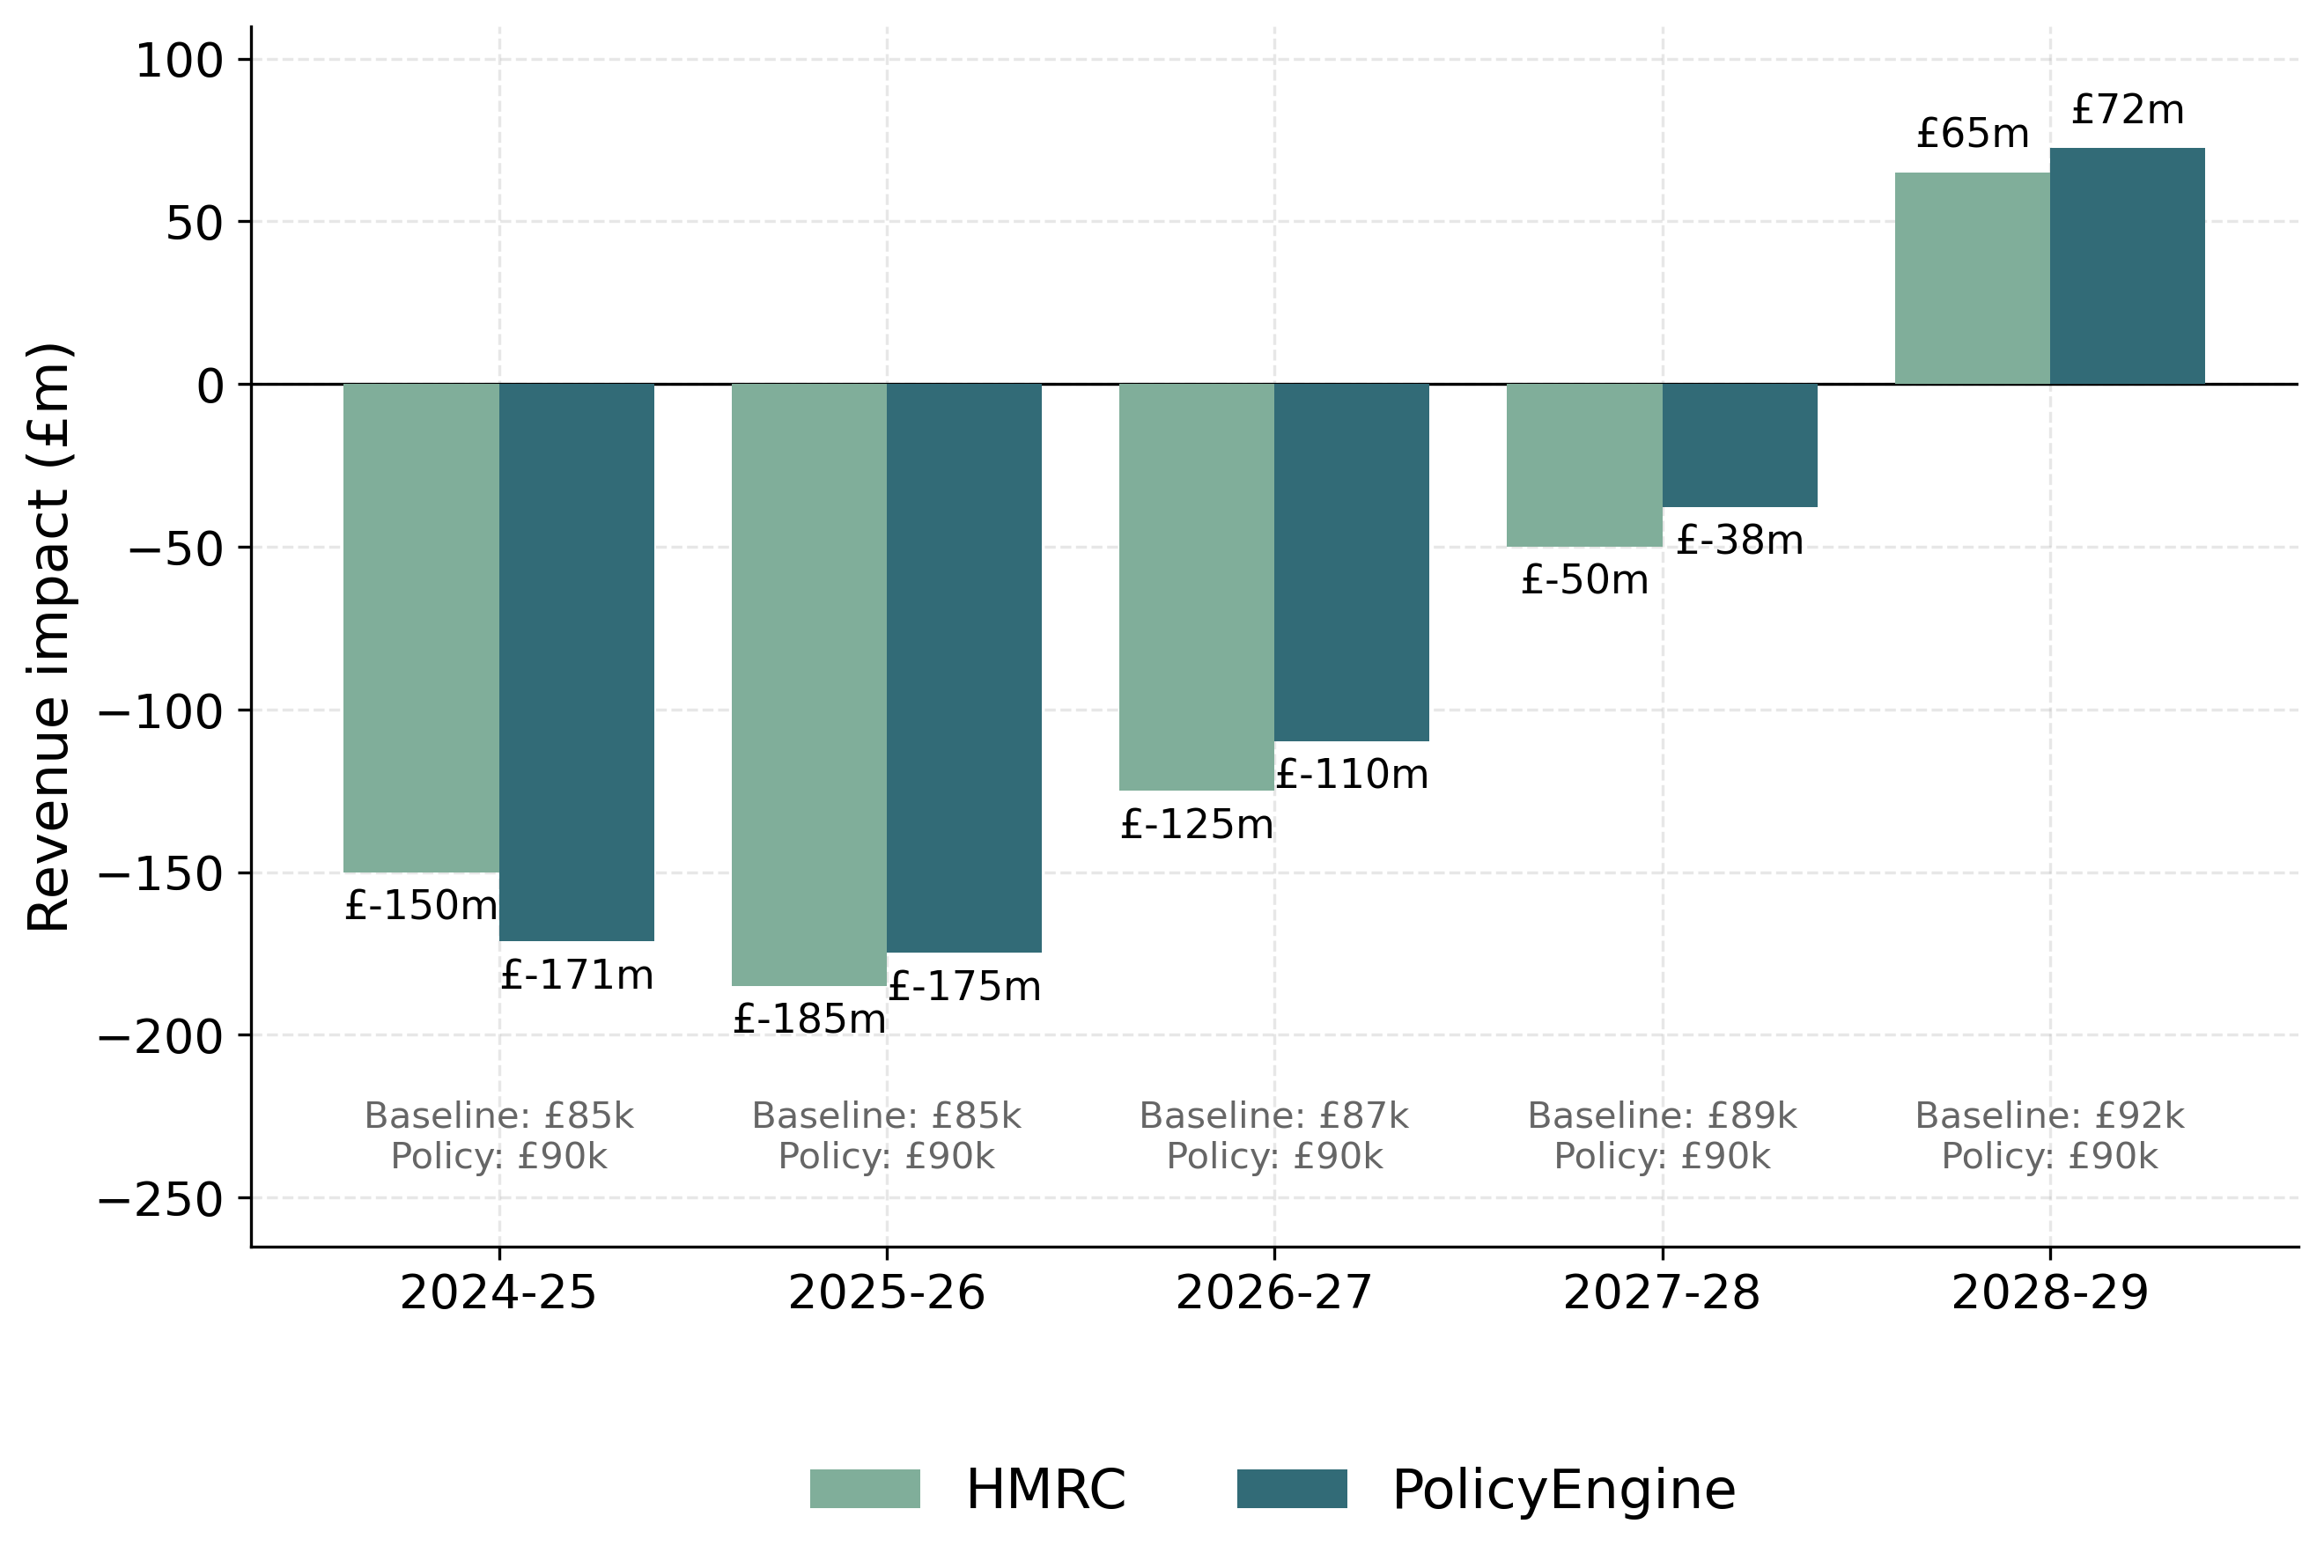
\includegraphics[width=0.78\textwidth]{figures/vat_threshold_revenue_impact.png}
\caption{Anchor reform: revenue impact of raising the VAT registration threshold
from \pounds85{,}000 to \pounds90{,}000 (the April~2024 change), my estimate
under the full-deregistration and 43\% retention conventions versus HMRC's
published costing, 2024--25 to 2028--29. Both series narrow over the
forecast and turn positive by 2028--29 because the costing baseline is a
counterfactual threshold path that resumes uprating after March~2026 and
overtakes \pounds90{,}000. The mechanical estimate, with no retention or
behavioural parameter, lies within 30\% of the official profile in each of
the four release years (within 10\% in 2025--26 and 2026--27) and 36\%
above it in the sign-flip year; the 43\% retention
convention undershoots it. Because the microdata are calibrated
to HMRC and OBR aggregates, this is a consistency check, not an out-of-sample
validation.}
\label{fig:hmrc_validation}
\end{figure}

\paragraph{A menu of threshold locations.} I next cost a menu of further threshold
locations, taking the post-reform \pounds90{,}000 threshold as the baseline. This
sweep runs on the 2024--25 vintage population (Section~\ref{sec:data}). Each
row of Table~\ref{tab:static_revenue} costs a move of the threshold to a new
location for 2025--26 by the registration rule above, holding the data-year
turnover distribution fixed, so the revenue change reflects only the
reclassification of in-scope firms into or out of the VAT net. Because the
optimiser determines the within-band shape near the threshold
(Section~\ref{sec:data}), and because the 2024--25 vintage has no fine-band
targets, so that its density steps at the \pounds90{,}000 HMRC band edge
(Section~\ref{sec:bunching}), the $\pm\pounds5{,}000$ rows are conditional on
that synthetic within-band allocation. Lowering the threshold draws in
in-scope firms not already registered---mainly the unregistered stratum, whose
liability under registration is the standard rate on its value added---while
raising it releases registered firms in the vacated band. A \pounds20{,}000
cut to \pounds70{,}000 raises about \pounds1.59bn and brings about 246{,}000
businesses into the net---at the standard rate on their modelled value added,
about \pounds6{,}400 per business; crediting them instead at HMRC's average
net remittance per registered below-threshold trader (\pounds2{,}152 in
2023--24) gives \pounds530m. A \pounds30{,}000 rise to \pounds120{,}000 costs
about \pounds1.28bn, 0.69\% of the \pounds184.1bn base. The cut rows
credit the full standard-rate liability of newly covered businesses, with no allowance for the compliance
cost or the registration lag a lower threshold would impose on them, and they
inherit the unregistered stratum's assumed exponential size distribution, so
they are illustrations of a maintained assumption rather than costings; the
per-firm-remittance variant above is the lower reading.
Figure~\ref{fig:static_sweep}
shows the sweep graphically. These are \emph{static} results: they bound the
first-order fiscal effect of a threshold change but abstract from the
behavioural response of Section~\ref{sec:behavioural}.

\begin{table}[htbp]
\centering
\caption{Static revenue and VAT-paying-firm effects of moving the VAT registration
threshold, 2025--26, relative to the post-reform \pounds90{,}000 baseline
(in-scope above-threshold VAT base \pounds184.1bn; 2024--25 vintage population).
Figures are mechanical, holding data-year turnover fixed (no behavioural
response); in-scope firms only, including the unregistered stratum below the
threshold. Voluntary registrants are held registered. Cut rows credit the full
liability of newly covered businesses (see text). This sweep is distinct from the anchor reform of
Figure~\ref{fig:hmrc_validation}. The machine-readable table is
\texttt{results/static\_sweep.txt} in the replication repository.}
\label{tab:static_revenue}
\begin{tabular}{lrrr}
\toprule
Threshold & Revenue change (\pounds m) & Change (\%) & VAT-paying firms (000s) \\
\midrule
\pounds70{,}000 & $+1{,}587.0$ & $+0.86$ & $+246.3$ \\
\pounds75{,}000 & $+1{,}171.0$ & $+0.64$ & $+175.3$ \\
\pounds80{,}000 & $+764.9$ & $+0.42$ & $+110.9$ \\
\pounds85{,}000 & $+376.5$ & $+0.20$ & $+52.7$ \\
\pounds90{,}000 (baseline) & $0$ & $0$ & $0$ \\
\pounds95{,}000 & $-198.0$ & $-0.11$ & $-28.8$ \\
\pounds100{,}000 & $-404.4$ & $-0.22$ & $-57.4$ \\
\pounds105{,}000 & $-625.9$ & $-0.34$ & $-86.3$ \\
\pounds110{,}000 & $-845.6$ & $-0.46$ & $-113.7$ \\
\pounds115{,}000 & $-1{,}066.0$ & $-0.58$ & $-139.6$ \\
\pounds120{,}000 & $-1{,}278.7$ & $-0.69$ & $-163.2$ \\
\bottomrule
\end{tabular}
\end{table}

\begin{figure}[htbp]
\centering
\subfigure[Revenue impact (\pounds m)]{%
    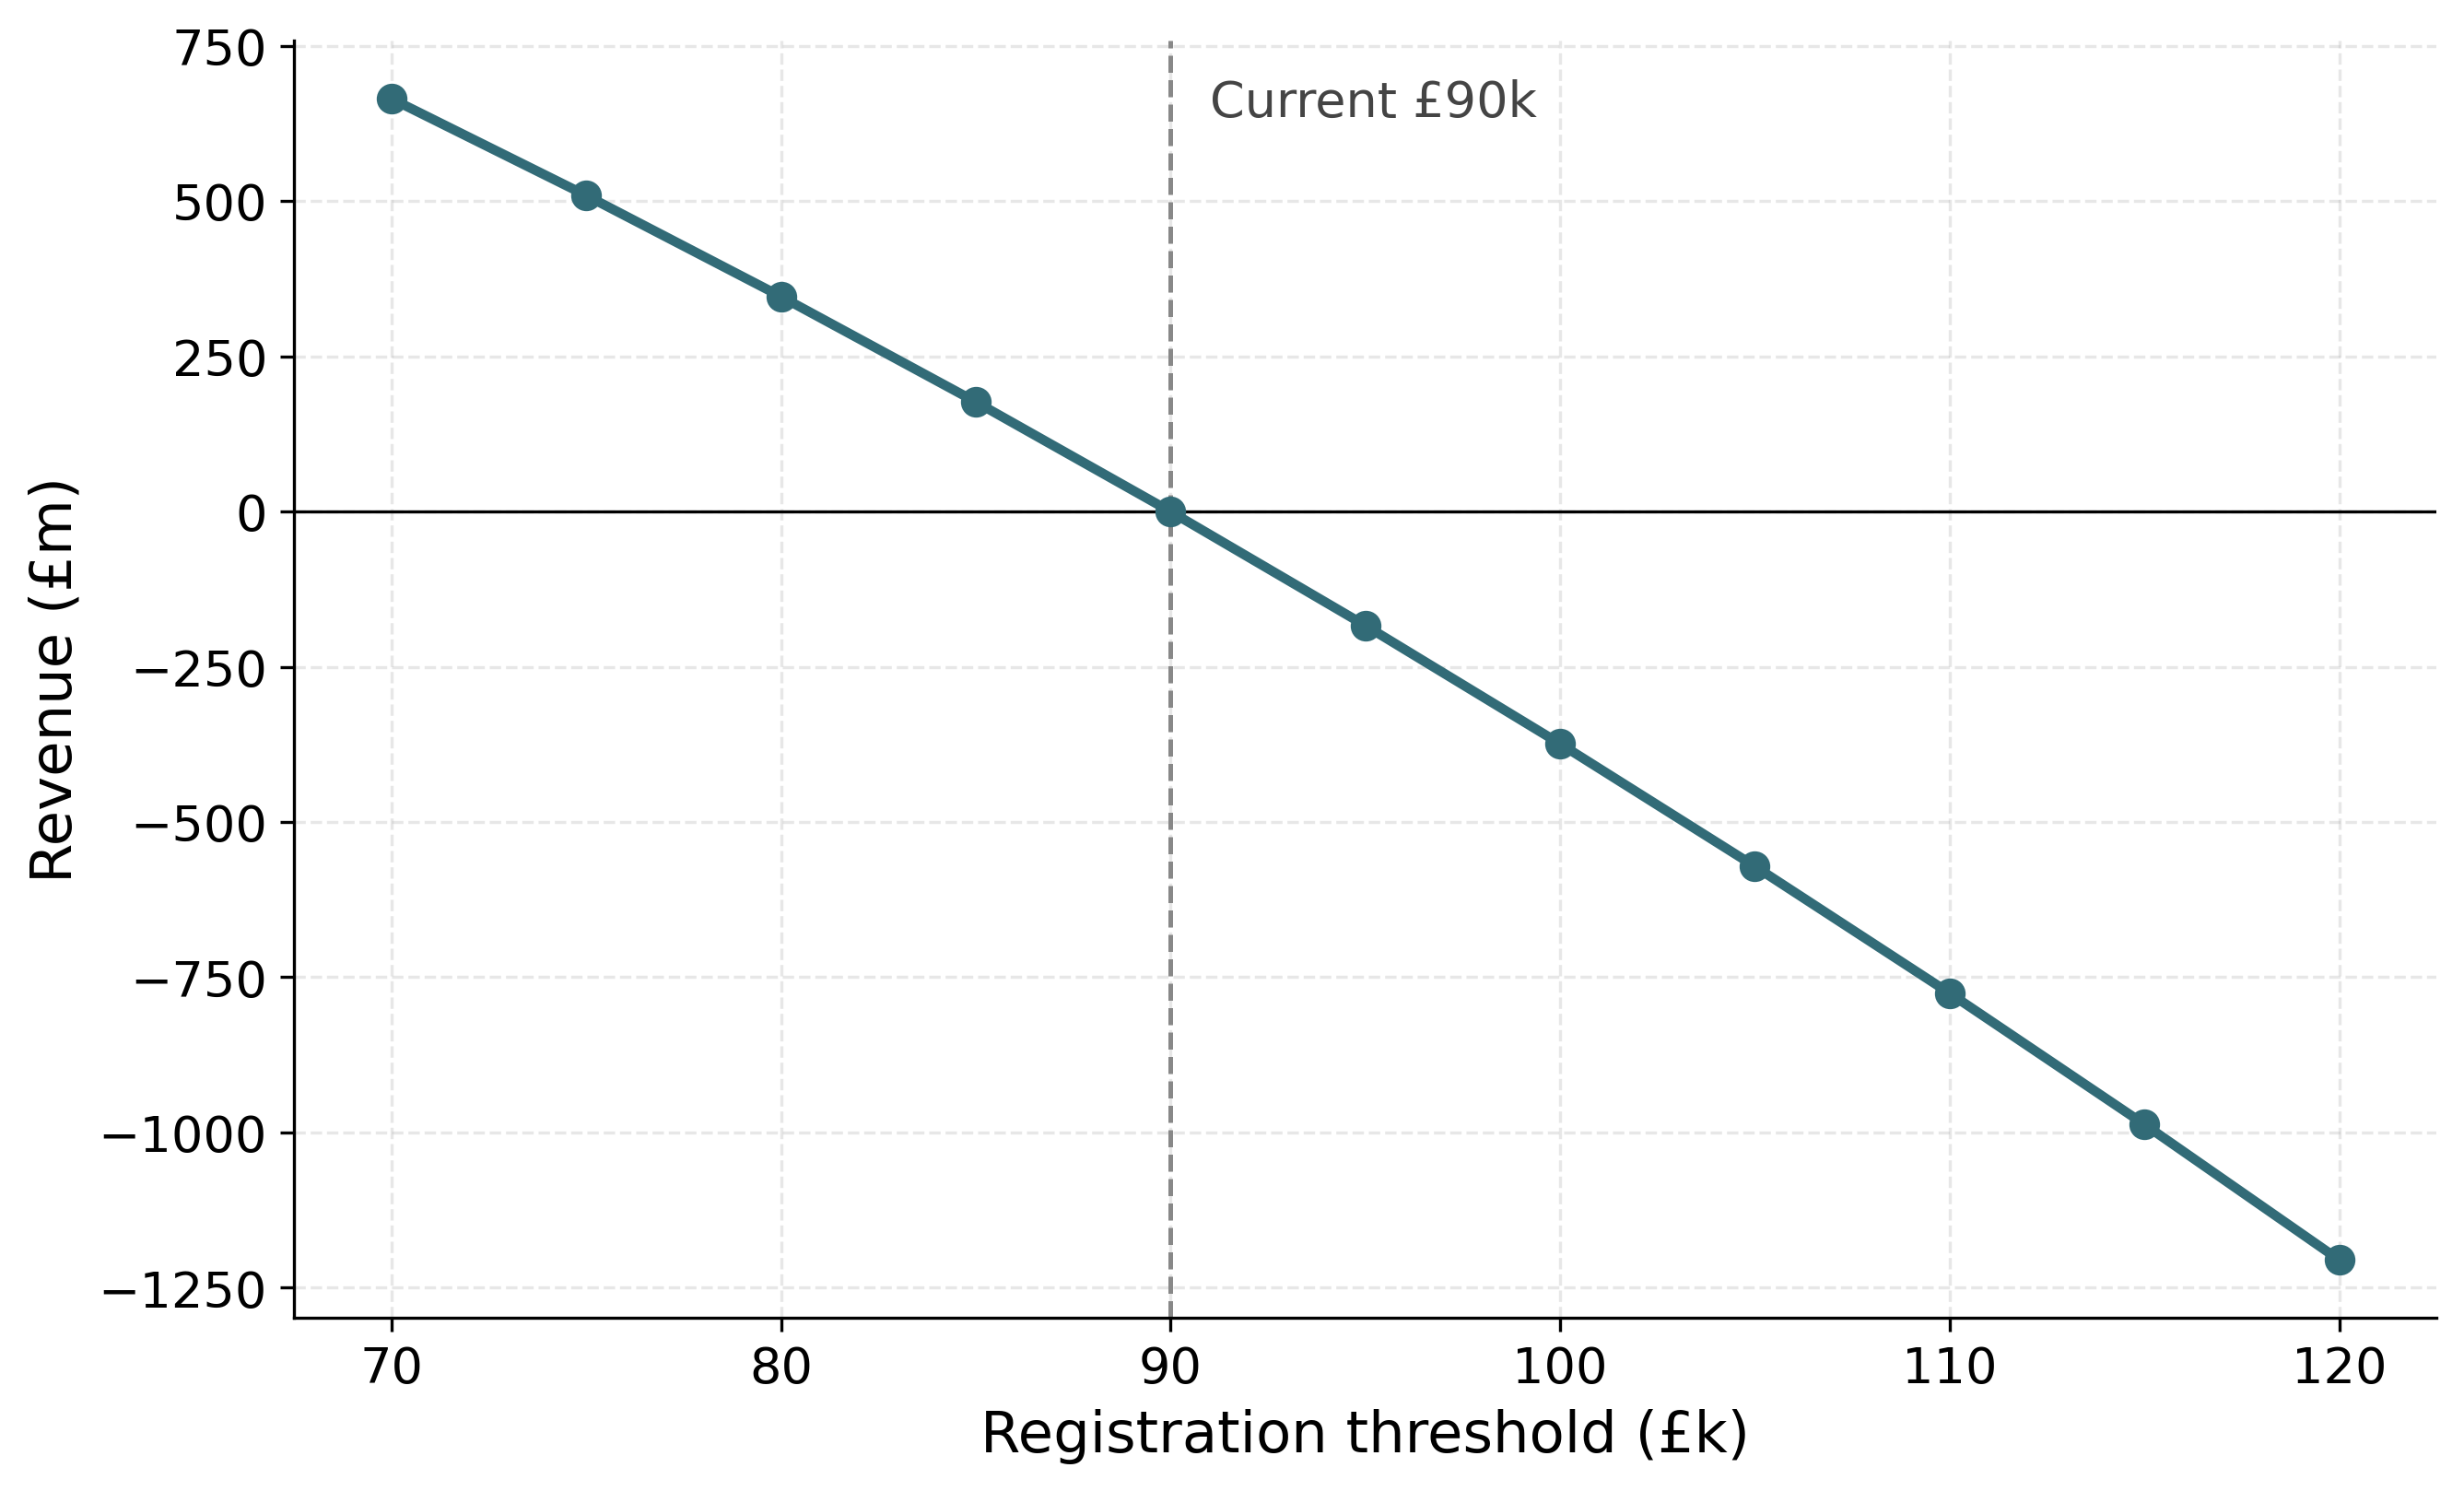
\includegraphics[width=0.48\textwidth]{figures/revenue_impact_2025_26.png}%
}\hfill%
\subfigure[Change in VAT-paying firms (000s)]{%
    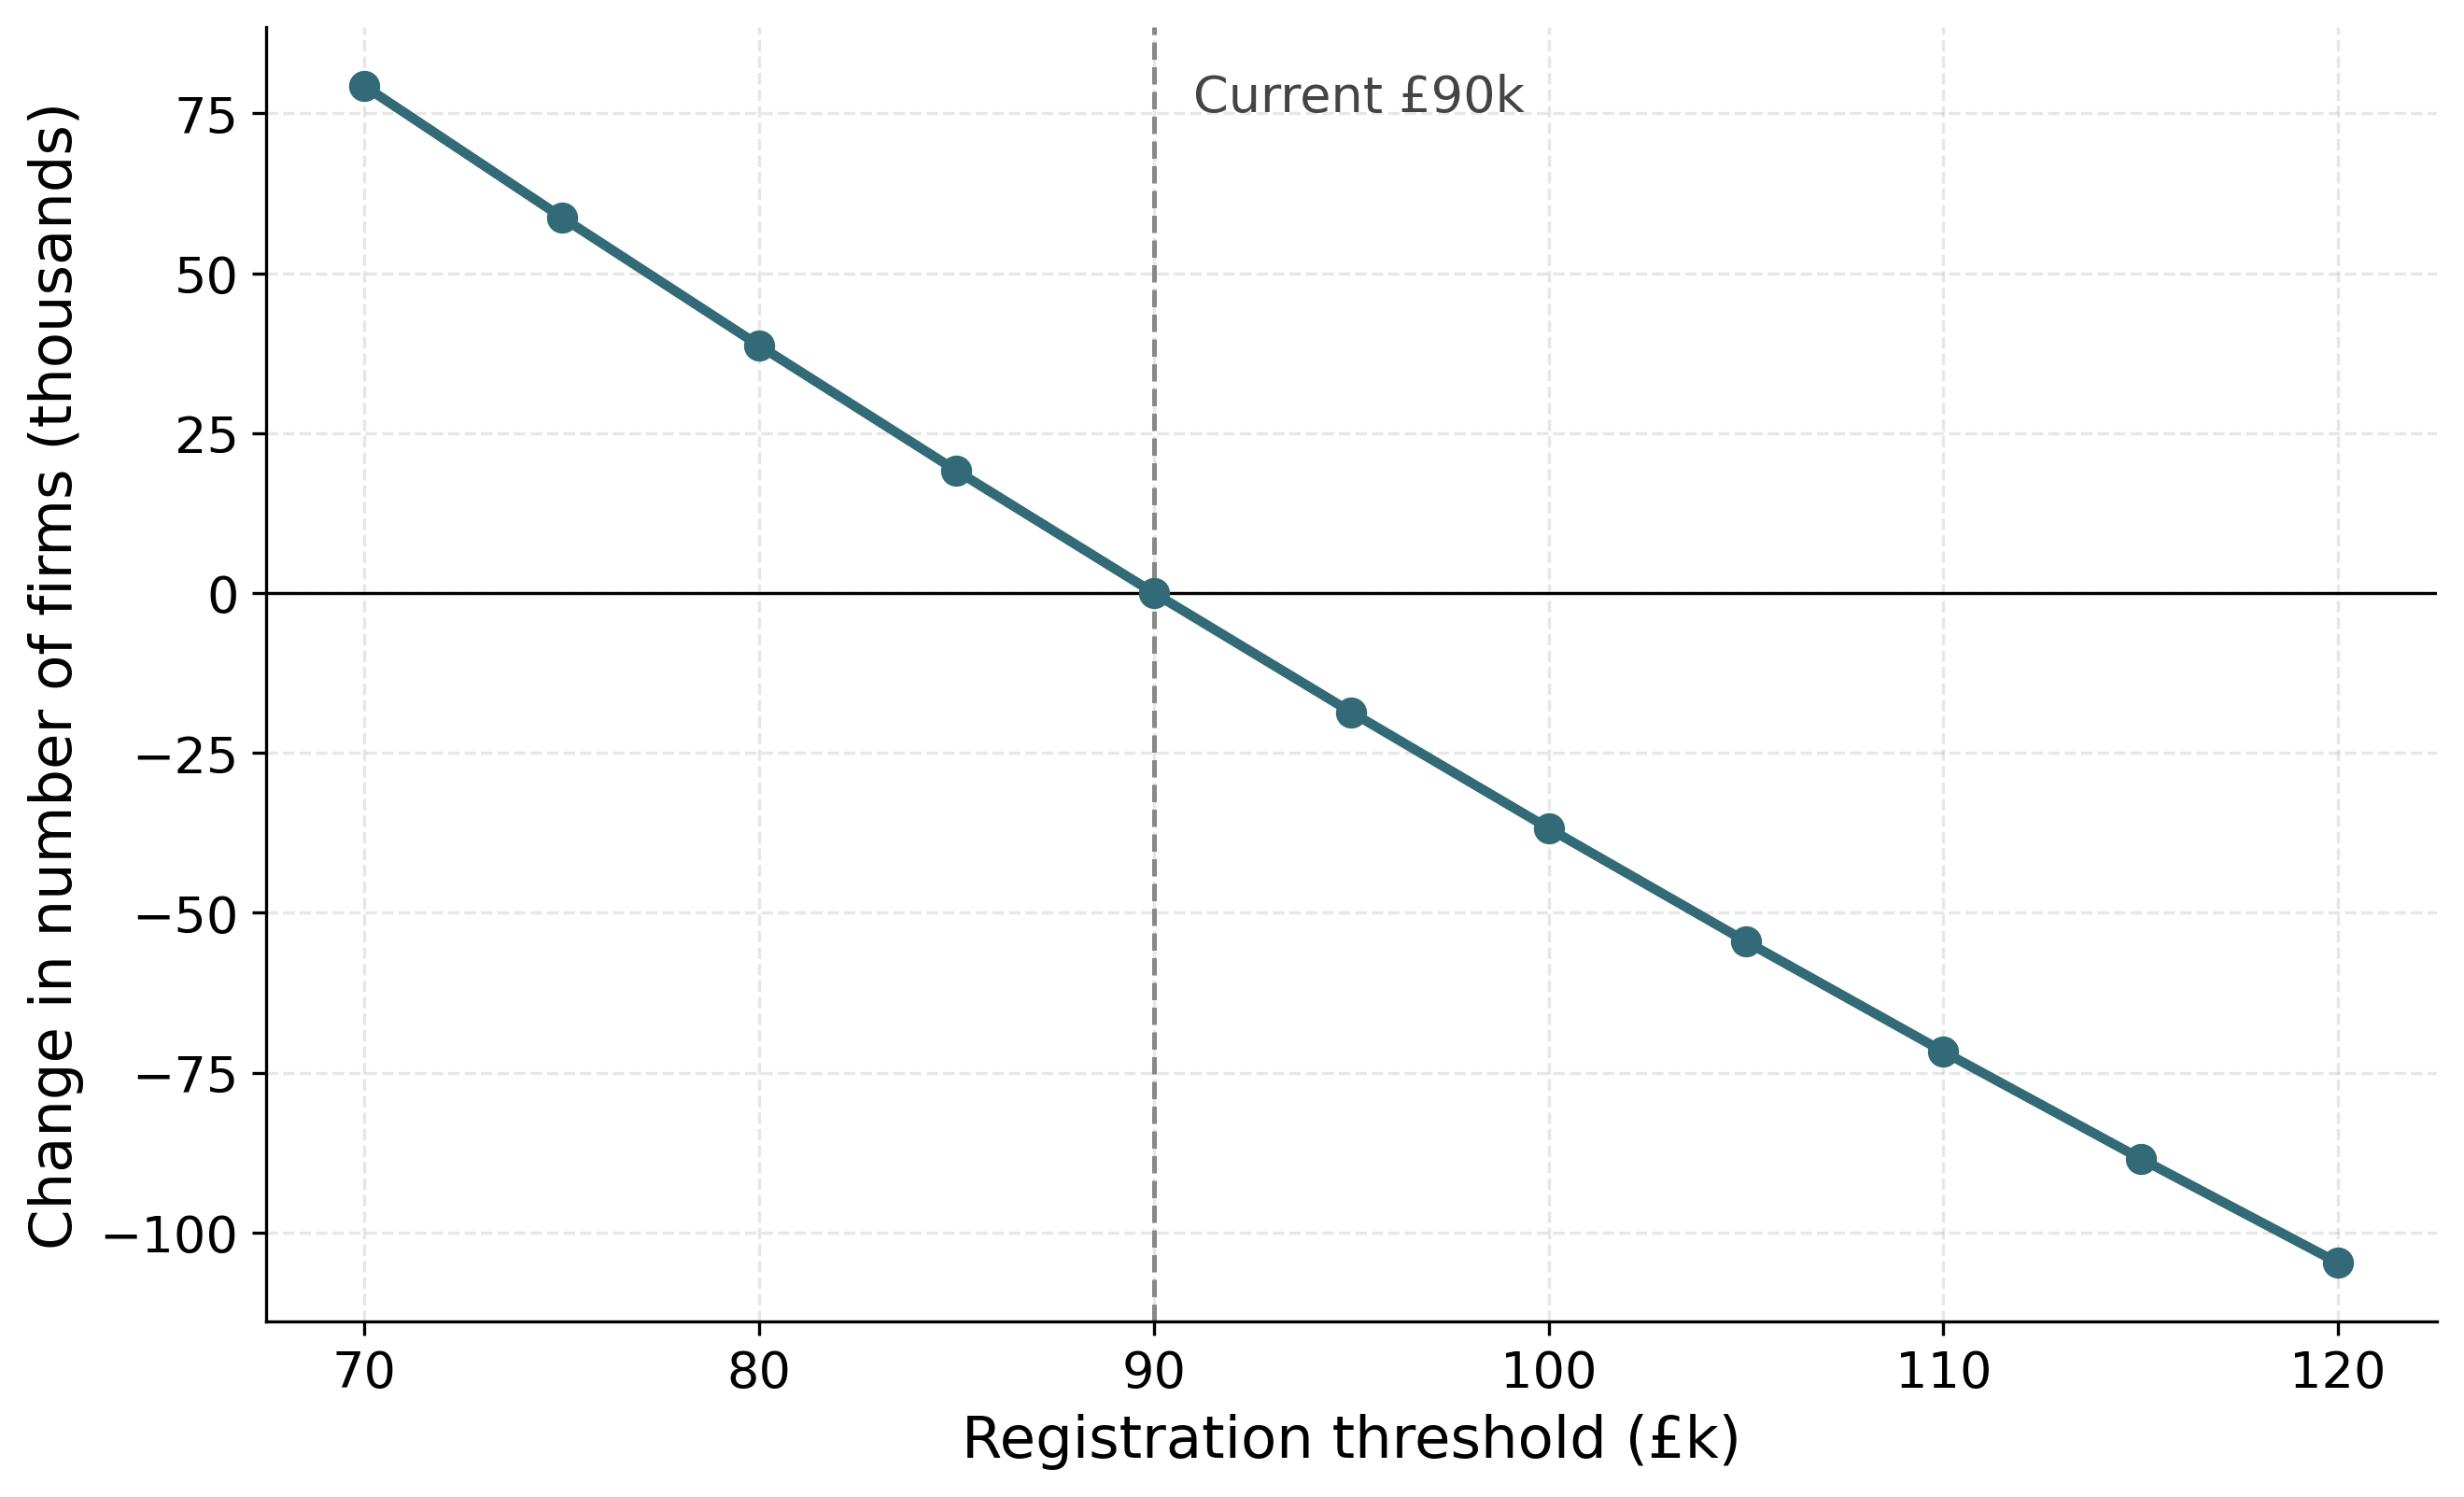
\includegraphics[width=0.48\textwidth]{figures/firms_impact_2025_26.png}%
}
\caption{Static effect of moving the VAT registration threshold, 2025--26, relative
to the \pounds90{,}000 baseline (dashed line). Panel (a): revenue impact---cuts
draw the unregistered stratum into the net; rises release registered firms.
Panel (b): the change in the
number of VAT-paying firms, tracking the local density of firms on each side of
the threshold.}
\label{fig:static_sweep}
\end{figure}

\subsection{Costing schedule reforms}
\label{ssec:schedule_costs}

The threshold sweep above moves the \emph{location} of a single cutoff. The same
static principle---re-applying a tax rule to the fixed turnover distribution, with
no behavioural response---also costs reforms that change the \emph{shape} of the
schedule rather than merely its position. I consider four reforms and report
their first-order revenue effects against a common baseline: the
\pounds85{,}000-notch / \pounds174.7bn 2023--24 base of in-scope firms. (This
2023--24 data-year base differs from the \pounds184.1bn figure in the sweep above, which runs on the
2024--25 vintage aged to 2025--26 at the post-reform \pounds90{,}000 threshold;
the schedule reforms are costed in the data year to match the bunching and
dominated-region analysis. Both bases are theoretical-liability (VTTL-style)
aggregates in the sense of the footnote above, not cash-receipts lines.) For each
reform I recompute the weighted sum of liabilities $R = \sum_i w_i\, v_i$ under
the new schedule, holding each firm's turnover fixed, and difference it against
the baseline.

\paragraph{Threshold relocation.} Raising the threshold from \pounds85{,}000 to
\pounds100{,}000 releases the firms with turnover in
$[\pounds85{,}000, \pounds100{,}000)$---about 87{,}800 in-scope
firms---from the VAT net, for a static revenue change of \(-\)\pounds583m on the
common base (the menu applies each schedule to in-scope firms at their data-year
turnover, without the deregistration-gap convention of the anchor). Because the
released band lies \emph{above} the data-year threshold, its liabilities are
directly calibrated (and its lower reach pinned by the OBR fine-band targets),
so the band is summed directly; a smooth-counterfactual alternative that fits
the above-threshold per-\pounds1{,}000 profile and integrates it across the
band gives \(-\)\pounds615m and 90{,}500 firms---within 6\% of the direct
sum now that the within-band fill is monotone. On this
common base the level move relocates the dominated region to the new cutoff and
widens it to \pounds25{,}000 (Section~\ref{sec:model}) at a static cost of
\(-\)\pounds583m; the linear taper removes the dominated region entirely at the
menu's largest static cost of \(-\)\pounds1{,}408m, and a constant-marginal-rate taper of
the same width does so at \(-\)\pounds932m (Section~\ref{sec:model}). Which matters more depends on what the
reader wants from the reform---the dominated-region metric indexes
misallocation only, and Section~\ref{sec:conclusion} discusses what it omits.

\paragraph{Graduated taper.} A graduated taper replaces the discrete notch with a
\emph{marginal} remittance rate that phases in over a band, so liability is the
integral of the marginal rate and a firm's \emph{effective} rate rises
continuously from $0\%$ to the full $20\%$ across the band. The band top is a
property of the chosen shape (Section~\ref{sec:model}): a taper whose marginal
rate is constant at $m>\tau$ meets the standard-rate line at
$U(m)=mT^{*}/(m-\tau)$, which is \pounds141{,}667 at $m=50\%$ and falls
towards \pounds106{,}250 as $m\to100\%$, while a taper reaching the full rate at
\pounds105{,}000 would push net revenue inside the band below its value at the
threshold, recreating a dominated interval smoothly rather than at a cliff. I
cost two designs on the same \pounds85{,}000--\pounds141{,}667 band: the
\emph{linear} taper, whose marginal rate rises from $0\%$ to $100\%$ across the
band, and a \emph{constant} $50\%$ marginal-rate taper. Firms in the band remit
the tapered schedule on their (fixed) turnover; mechanically the linear design
reduces revenue by \(-\)\pounds1{,}408m and the constant-rate design by \(-\)\pounds932m, with
about 278{,}100 in-scope firms in the band facing a lower effective rate.
The linear design gives more relief low in the band at the price of a marginal
remittance rate that reaches $100\%$ at the top; the constant-rate design caps
the marginal rate at $50\%$ and costs a third less.

\paragraph{Banded reduced rate.} A banded reduced rate charges firms in the
\pounds85{,}000--\pounds105{,}000 band a reduced rate
$\tau_{\text{low}}\in\{10\%,15\%\}$ in place of the standard $20\%$, with $20\%$
retained above \pounds105{,}000. Statically this reduces revenue by \(-\)\pounds398m
at $\tau_{\text{low}}=10\%$ and by \(-\)\pounds199m at $\tau_{\text{low}}=15\%$,
with about 117{,}300 in-scope firms in the band facing the lower rate.

\begin{table}[htbp]
\centering
\caption{Static, behaviour-free revenue effect of the reforms relative to the
common \pounds85{,}000-notch / \pounds174.7bn 2023--24 baseline of in-scope
firms. Each reform is costed mechanically by re-applying its schedule to the
fixed turnover distribution, with no behavioural response.}
\label{tab:schedule_costs}
\small
\begin{tabularx}{\textwidth}{@{}Xlr@{}}
\toprule
Reform & Lever & Static (\pounds m) \\
\midrule
Raise threshold to \pounds100{,}000 & Location & $-583$ \\
Linear taper, \pounds85k--\pounds141.7k & Shape (marginal rate $0\to100\%$) & $-1{,}408$ \\
Constant $50\%$ marginal taper, \pounds85k--\pounds141.7k & Shape (marginal rate $50\%$) & $-932$ \\
Reduced rate $10\%$, \pounds85k--\pounds105k & Rate (step) & $-398$ \\
Reduced rate $15\%$, \pounds85k--\pounds105k & Rate (step) & $-199$ \\
\bottomrule
\end{tabularx}
\end{table}

These static figures bound the first-order fiscal effect of each reform but
abstract from the behavioural response of Section~\ref{sec:behavioural}. Two
maintained conventions carry through every costing: the firm bears the full
statutory rate on its value added (no pass-through to prices), and per-firm
liability is the standard rate on value added, so Flat Rate Scheme users---who
are concentrated in exactly the \pounds85{,}000--\pounds150{,}000 bands---are
represented only through the calibrated band totals, not individually. One feature
of the shape reforms is not visible in a static costing: unlike a threshold move,
which transports the notch to a new cutoff, the taper and the reduced rate
\emph{change the size of the notch itself}---the discrete drop in net revenue at the
threshold and the empty band of turnover it induces. Quantifying that change
requires the structural object I develop in Section~\ref{sec:model}, where I derive
the notch's dominated region and show analytically how each of these reforms alters
it.


\newpage
\bibliographystyle{econ}
{\small \bibliography{references}}

\end{document}
